\documentclass[xcolor=dvipsnames]{beamer}
%\documentclass[pdftex,hyperref={colorlinks=false}]{beamer}
%\documentclass[handout,xcolor=dvipsnames,pdftex,hyperref={colorlinks=false}]{beamer}

% == Packages for beamer
\usepackage{xcolor}
\usepackage{graphicx}
\usepackage{fancybox}
\usepackage{hyperref}
\usepackage{amsmath,amssymb,amsfonts,bm}
\usepackage{wasysym}
\usepackage{colortbl}
\usepackage[english]{babel}
\usepackage{times}
\usepackage[T1]{fontenc}
\usepackage{multirow}

% == Other Packages
\usepackage{rotating}
\usepackage{latexsym}
\usepackage{ulem}

\newenvironment{Shaded}{}{}


% == theme & colors
\usetheme{Warsaw}  % Jens' previous
\usepackage{helvet}
\definecolor{someblue}{rgb}{0,.1,0.8}

% == New Commands
% = For general typesetting
\newcommand\spacingset[1]{\renewcommand{\baselinestretch}{#1}\small\normalsize}
\renewcommand\r{\right}
\renewcommand\l{\left}

\newcommand\makegaps{\addtolength{\itemsep}{.25\baselineskip}}
\newcommand\makebiggaps{\addtolength{\itemsep}{.5\baselineskip}}
\newcommand\smallunskip{\vspace{-.25\baselineskip}}
\newcommand\medunskip{\vspace{-.5\baselineskip}}
\newcommand\bigunskip{\vspace{-\baselineskip}}

\newcommand{\VerbBar}{|}
\newcommand{\VERB}{\Verb[commandchars=\\\{\}]}
% Add ',fontsize=\small' for more characters per line
\newcommand{\KeywordTok}[1]{\textcolor[rgb]{0.00,0.44,0.13}{\textbf{{#1}}}}
\newcommand{\DataTypeTok}[1]{\textcolor[rgb]{0.56,0.13,0.00}{{#1}}}
\newcommand{\DecValTok}[1]{\textcolor[rgb]{0.25,0.63,0.44}{{#1}}}
\newcommand{\BaseNTok}[1]{\textcolor[rgb]{0.25,0.63,0.44}{{#1}}}
\newcommand{\FloatTok}[1]{\textcolor[rgb]{0.25,0.63,0.44}{{#1}}}
\newcommand{\CharTok}[1]{\textcolor[rgb]{0.25,0.44,0.63}{{#1}}}
\newcommand{\StringTok}[1]{\textcolor[rgb]{0.25,0.44,0.63}{{#1}}}
\newcommand{\CommentTok}[1]{\textcolor[rgb]{0.38,0.63,0.69}{\textit{{#1}}}}
\newcommand{\OtherTok}[1]{\textcolor[rgb]{0.00,0.44,0.13}{{#1}}}
\newcommand{\AlertTok}[1]{\textcolor[rgb]{1.00,0.00,0.00}{\textbf{{#1}}}}
\newcommand{\FunctionTok}[1]{\textcolor[rgb]{0.02,0.16,0.49}{{#1}}}
\newcommand{\RegionMarkerTok}[1]{{#1}}
\newcommand{\ErrorTok}[1]{\textcolor[rgb]{1.00,0.00,0.00}{\textbf{{#1}}}}
\newcommand{\NormalTok}[1]{{#1}}


% = For stats & econometrics
\renewcommand{\epsilon}{\varepsilon}
\newcommand\ud{\mathrm{d}}
\newcommand\dist{\buildrel\rm d\over\sim}
\newcommand\ind{\stackrel{\rm indep.}{\sim}}
\newcommand\iid{\stackrel{\rm i.i.d.}{\sim}}
\newcommand\logit{{\rm logit}}
\newcommand\cA{\mathcal{A}}
\newcommand\cN{\mathcal{N}}
\newcommand\E{\mathbb{E}}
\newcommand\V{\mathbb{V}}
\newcommand\cJ{\mathcal{J}}
\newcommand\y{{\bm y}}
\newcommand\Y{{\bm Y}}
\newcommand\X{{\bm X}}
\newcommand\x{{\bm x}}
\newcommand\eps{{\bm\varepsilon}}
\newcommand\zero{{\bm 0}}
\newcommand\be{{\bm\beta}}
\renewcommand\b{{\bm b}}
\newcommand\C{{\bm C}}
\newcommand\D{{\bm D}}
\newcommand\I{{\bm I}}
\newcommand\Z{{\bm Z}}
\newcommand\eeta{{\bm \eta}}
\newcommand{\Var}{\mathrm{Var}}
\newcommand{\Cov}{\mathrm{Cov}}

\DeclareMathOperator*\plim{plim}
\DeclareMathOperator\rank{rank}
\newcommand\indep{\protect\mathpalette{\protect\independenT}{\perp}}
\DeclareMathOperator{\sgn}{sgn}
\def\independenT#1#2{\mathrel{\rlap{$#1#2$}\mkern2mu{#1#2}}}

%\documentclass[xcolor=dvipsnames]{beamer}
%%\usecolortheme[named=OliveGreen]{structure}
%\usecolortheme[named=Blue]{structure}
%%\usetheme{Rochester}
%\setbeamertemplate{items}[ball]
%\setbeamertemplate{blocks}[rounded][shadow=true]
%\usepackage{xcolor}
%\usepackage{colortbl}
%\setbeamertemplate{navigation symbols}{}
%\usepackage{amssymb}
%\usepackage{amsmath}
%\usepackage[english]{babel}
%% or whatever
%
%%\usepackage[latin1]{inputenc}
%% or whatever
%
%%\mode<presentation>
%%{
%\usetheme{Warsaw}
%  % or ...
%  %\usecolorheme{albatross}
%%  \setbeamercovered{transparent}
%  % or whatever (possibly just delete it)
%%}

%\usepackage{helvet}
%%\usepackage[T1]{fontenc}
%% Or whatever. Note that the encoding and the font should match. If T1
%% does not look nice, try deleting the line with the fontenc.

\newtheorem{assumption}{Assumption}
\newtheorem{iass}{Identification Assumption}
\newtheorem{ires}{Identfication Result}
\newtheorem{estm}{Estimand}
\newtheorem{esti}{Estimator}

%\newcommand{\indep}{{\bot\negthickspace\negthickspace\bot}}
\newcommand{\notindep}{{\bot\negthickspace\negthickspace\bot}{\negthinspace
  \negmedspace \negthickspace \negthickspace \diagup
  \;}}

\newcommand{\bs}{\boldsymbol}
\newcommand{\mb}{\mathbf}
\newcommand{\real}{\mathbb{R}}
\renewcommand{\u}{\ensuremath{\mb{u}}}
\renewcommand{\v}{\ensuremath{\mb{v}}}
\newcommand{\U}{\ensuremath{\mb{U}}}
\newcommand{\M}{\ensuremath{\mb{M}}}
\renewcommand{\b}{\ensuremath{\bs{\beta}}}
\newcommand{\e}{\ensuremath{\bs{\epsilon}}}
\newcommand{\bhat}{\ensuremath{\hat{\bs{\beta}}}}
\newcommand{\XX}{\ensuremath{\X'\X}}
\newcommand{\XXinv}{\ensuremath{\left(\XX\right)^{-1}}}
\newcommand{\hatsig}{\ensuremath{\hat{\sigma}^2}}
\newcommand{\sig}{\ensuremath{\sigma^2}}
\newcommand{\hatmat}{\ensuremath{\X \XXinv \X'}}
\newcommand{\ehat}{\ensuremath{\hat{\e}}}
\newcommand{\tr}{\text{tr}}
\newcommand{\Sig}{\ensuremath{\bs{\Sigma}}}
\newcommand{\SigInv}{\ensuremath{\bs{\Sigma^{-1}}}}
\newcommand{\W}{\ensuremath{\mb{W}}}

%\usepackage{fixltx2e} % provides \textsubscript
%\ifxetex
%%  \usepackage{fontspec,xltxtra,xunicode}
%  \usepackage{mathspec,xltxtra,xunicode}
%  \defaultfontfeatures{Mapping=tex-text,Scale=MatchLowercase}
%  \setmainfont[Ligatures={Common,TeX}]{Gill Sans}
% % \setmathfont[Digits, Latin]{Gill Sans}
% \setmathfont{LucidaBrightMathOT.otf}
%
%\else
%  \ifluatex
%    \usepackage{fontspec}
%    \defaultfontfeatures{Mapping=tex-text,Scale=MatchLowercase}
%  \else
%    \usepackage[utf8]{inputenc}
%  \fi
%\fi

\AtBeginSection[]
{
  \begin{frame}<beamer>
    \frametitle{Outline}
    \tableofcontents[currentsection]
  \end{frame}
}
%\AtBeginSubsection[]
%{
%  \begin{frame}<beamer>
%    \frametitle{Outline}
%    \tableofcontents[currentsection,currentsubsection]
%  \end{frame}
%}

\title[]{Selection on Observables I \\ \small Identification and Sub-Classification}
\subtitle[ ]{PS200C, Spring 2024}
\author[Hazlett]{Chad Hazlett }
\institute[UCLA]{UCLA\\[1ex]
  \texttt{chazlett@ucla.edu}
}
\date{}

\definecolor{dgreen}{rgb}{0,.6,0.8}
\useoutertheme{infolines}

\begin{document}

\subject{Talks}
\AtBeginSection[]
{
  \begin{frame}<beamer>
    \frametitle{Outline}
    \tableofcontents[currentsection]
  \end{frame}
}

%\AtBeginSubsection[]
%{
%  \begin{frame}<beamer>
%    \frametitle{Outline}
%    \tableofcontents[currentsection,currentsubsection]
%  \end{frame}
%}

\begin{frame}
  \titlepage
\end{frame}


\begin{frame}{Observational Studies}
\small
\begin{itemize}
\itemsep1pt\parskip5pt\parsep0pt
\item Randomization allows unbiased estimation of $\E[Y_{0i}|D_i=1]$ via $\E[Y_{0i}|D_i=0]$ and $\E[Y_{1i}|D_i=0]$ via $\E[Y_{1i}|D_i=1]$.
\begin{itemize}
\footnotesize
\item<2->[] \textcolor{Blue}{Equivalently}: We can think about influences on POs rather than the POs, with randomzation ``balancing'' \alert{observed} and \alert{unobserved} influences on POs 
\end{itemize}
\small
\item<3-> When we cannot randomize, we do observational studies, primarily meaning we \alert{adjust} for \alert{observed covariates} and \alert{hope} that unobservables are balanced 
\end{itemize}
\bigskip
\onslide<4-> Most of the rest of the course: what to do in observational settings. 
\footnotesize
\begin{itemize}
\item<5-> What is your strategy for identifying the missing potential outcomes from observational data? 
\item<5-> What assumptions does it involve? Can we weaken these?
\item<5-> Are they credible? What can you test? What do you need to argue? 
\end{itemize}
\end{frame}

\section*{What Makes a Good Observational
Study?}\label{what-makes-a-good-observational-study}
%
%\begin{frame}{The Good, the Bad, and the Ugly}
%\textbf{Treatments, Covariates, Outcomes}
%\small
%\begin{itemize}
%\itemsep1pt\parskip0pt\parsep0pt
%\item<1->
%  \alert{Randomized Experiment}: Well-defined treatment, clear
%  distinction between covariates and outcomes, control of assignment mechanism\medskip
%\item<2->
%  \alert{Better Observational Study}: Well-defined treatment, clear
%  distinction between covariates and outcomes, precise knowledge of assignment mechanism\
%
%  \begin{itemize}
%\footnotesize  
%    \item[]
%    Can convincingly answer the following question: Why do two units who
%    are identical on measured covariates receive different treatments?
%  \end{itemize}
%\small
%\item<3->
%  \alert{Poorer Observational Study}: Distinction between covariates and
%  outcomes is blurred. No precise knowledge of assignment mechanism
%\end{itemize}
%\end{frame}

%
%\begin{frame}{The Good, the Bad, and the Ugly}
%\textbf{How were treatments assigned?}
%\medskip
%\small
%\begin{itemize}
%\itemsep1pt\parskip10pt\parsep0pt
%\item<1->
%  \alert{Randomized Experiment}: Random assignment \medskip
%\item<2->
%  \alert{Better Observational Study}: Assignment is not random, but circumstances for the study were chosen so that, at least within some groups, we think treatment was not related to potential outcomes (see natural or quasi-experiments) \medskip
%\item<3-> \alert{Poorer Observational Study}: Little attention given to assignment process, units may self-select into treatment based on potential outcomes
%\end{itemize}
%\end{frame}

%\begin{frame}{The Good, the Bad, and the Ugly}
%\textbf{What is the problem with purely cross-sectional data?}
%
%\begin{itemize}
%\itemsep1pt\parskip0pt\parsep0pt
%\item
%  Difficult to know what is pre or post treatment. \medskip
%\item
%  Many important confounders will be affected by the treatment and including these ``bad controls'' induces post-treatment bias. \medskip
%\item
%  But if you do not condition on the confounders that are
%  post-treatment, then often only left with a limited set of covariates
%  such as socio-demographics.
%\end{itemize}
%\end{frame}
%
%\begin{frame}{The Good, the Bad, and the Ugly}
%
%\textbf{Were treated and controls comparable?}
%
%\begin{itemize}
%\item \alert{Randomized Experiment}: Balance table for observables. 
%\bigskip
%\item \alert{Better Observational Study}: Balance table for observables. Ideally sensitivity analysis for unobservables. \bigskip
%\item \alert{Poorer Observational Study}: No direct assessment of comparability is presented.
%\end{itemize}
%\end{frame}
%
%\begin{frame}{The Good, the Bad, and the Ugly}
%
%\textbf{Eliminating plausible alternatives to treatment effects?}
%\bigskip
%\small
%\begin{itemize}
%\item<1-> \alert{Randomized Experiment}: List plausible alternatives, if any. Design attempts to avoid or shed light on possible alternatives (e.g. placebos, multiple treatments, monitoring of treatment, multiple measures). Report on potential attrition and non-compliance,
% \bigskip
%\item<2-> \alert{Better Observational Study}: List plausible alternatives and study design includes features that shed light on these alternatives (e.g. multiple control groups, longitudinal covariate data, etc.). Rules out some alternatives, examines sensitivitiy. Requires more work than experiment since more alternatives. 
%\bigskip
%\item<3-> \alert{Poorer Observational Study}: Alternatives mentioned in discussion section only or not at all. Over-sells causal claim. 
%\end{itemize}
%\end{frame}

\begin{frame}{Good Observational Studies}
\alert{Preview:} Some designs we will introduce:
\bigskip
\footnotesize
\begin{itemize}
\item<1-> ``Finding experiments'' in the data: constructing comparison groups s.t. treatment assignment arguably haphazard.  \textcolor{Blue}{Keywords}:  conditional ignorability, controlling for common causes, no unobserved confounders, selection on observables.   
\medskip
\item<2-> Over-time comparisons to remove time-invariant confounders. \textcolor{Blue}{Keywords}: Fixed effects
\medskip
\item<3-> Over-time and between group comparisons to remove time-invariant effects and effects of time. \textcolor{Blue}{Keywords}: Diff-in-Diff, panel, synthetic control  \medskip
\item<4-> Finding surrogates for treatment or ``the random component'' of treatment \textcolor{Blue}{Keywords}: Instrumental variables.
\medskip
\item<5-> Leveraging sudden changes. \textcolor{Blue}{Keywords}: Regression discontinuity, interupted time-series. \medskip
\item<6-> Leveraging over time changes in treatment availability, while allowing selection-into-treatment. \textcolor{Blue}{Keywords:} Stability controlled quasi-experiment.
\medskip
\item<6-> Allow violated assumptions but clarify how violated they would have to be to alter conclusion. \textcolor{Blue}{Keywords:} Sensitivity analyses.
\end{itemize}
\end{frame}

\begin{frame}{The First Commandment of Causal Inference}

\onslide<1->
\begin{center}
\textcolor{Red}{A result is causal if you can support the assumptions that make it causal, not because you performed some procedure.}
\end{center}

\bigskip
\footnotesize
\begin{itemize}
\item talking about and learning estimation tools is great but no estimation tool \textbf{makes} your result causal; rather the assumptions tell you what you'd have to believe to believe the result is causal.
\item under a given set of assumptions, a variety of estimators may be suitable and the choice may matter less than the credibility rooted in the assumptions.
\item \textcolor{Red}{most of your effort should go into finding an ID strategy with the most suitable assumptions for your case, then understanding and communicating whether the assumptions are credible or how violations may have changed conclusion.}
\end{itemize}
\end{frame}

\begin{frame}
\begin{center}
\onslide<1-> \textcolor{Blue}{Corollary to First Commandment}: \\
 \textcolor{Red}{Never say ``my estimate is causal because I used [estimator].''} \\ \footnotesize (Where [estimator]=matching, IV, whatever.)
\end{center}
\end{frame}

%\begin{frame}{Good Observational Studies}
%\begin{enumerate}
%\def\labelenumi{\arabic{enumi}.}
%\itemsep1pt\parskip0pt\parsep0pt
%\item
%  An observational study should be structured to resemble an experiment.\medskip
%\item
%  Adjustment for observed covariates should be simple, transparent, and
%  convincing.\medskip
%\item
%  The most plausible alternatives to the treatment effect should be
%  anticipated and addressed.\medskip
%\item
%  The analysis should address possible biases from unmeasured
%  covariates.
%%\item There should be a plan for a primary analysis.
%\end{enumerate}
%
%\end{frame}

\section{Our first non-random ID Strategy: CI/SOO}

\begin{frame}
\frametitle{Setting}
\small
\vspace{-.25\baselineskip}
\begin{itemize}
\item<1-> Units: $i = 1, ..., n$
\item<1-> Treatment: $D_i \in \{0,1\}$
\item<1-> Potential outcomes: $Y_{di}$, where $d = \{0,1\}$
\smallskip
\item<2-> Quantities of interest:
\begin{eqnarray*}
\text{ATE:} \quad \tau_{ATE} & \equiv & \E[Y_{1i} - Y_{0i}] \\
\text{ATT:} \quad \tau_{ATT} & \equiv & \E[Y_{1i} - Y_{0i} \mid D_i=1] 
\end{eqnarray*}
\smallskip
\item<3-> \alert{Pre-treatment covariates}: $X_i = [X_{i1}, ..., X_{iK}]^\top \in \mathcal{X}$
	\begin{itemize}
	\footnotesize
	\addtolength{\itemsep}{.25\baselineskip}
	\item Examples: Sex, race, age, etc.
	\item $X_i$ may be correlated with both $D_i$ and $Y_{di}$, thereby \alert{confounding} the causal relationship \pause
	\item For now, take care that the covariates are not affected by $D_i$, but there are some other trouble cases we will get to with DAGs.
	\end{itemize}
\end{itemize}

\end{frame}


\begin{frame}
\frametitle{Conditional Ignorability/ Selection on Observables}
\small
\onslide<1-> Recall that randomized experiments work because:\\
$$ \{ Y_{0i}, Y_{1i}\} \ \indep \ D_i $$

\onslide<2-> Let's change it a bit:\\
\begin{block}{Assumption: Conditional Ignorability}
$$ \{ Y_{0i}, Y_{1i}\} \ \indep \ D_i \mid X_i = x \quad \text{for any} \quad x \in \mathcal{X} $$
\smallskip
\footnotesize
This goes by many names: strong ignorability, unconfoundedness, selection on observables, conditionally as-if random, no omitted variables \\
\end{block}
\smallskip
\onslide<3-> Tip: Read it backwards...```Among units with same $X$, $D_i$ is (as good as) randomly assigned.''
\end{frame}

\begin{frame}
\frametitle{Conditional Ignorability/ Selection on Observables}
\small
\onslide<1-> What does it really mean?
\begin{block}{Assumption: Conditional Ignorability}
$$ \{ Y_{0i}, Y_{1i}\} \ \indep \ D_i \mid X_i = x \quad \text{for any} \quad x \in \mathcal{X} $$
\end{block}
\smallskip
\footnotesize
This \textit{would be satisfied by design} if you performed ``conditional experiments'': imagine taking units with some value of $X$ and conducting a randomized experiment with them ($Pr(D)$ can vary by group).
\scriptsize
\begin{itemize} 
\item<2-> While one could run an experiment this way, this will get applied to observational studies where nobody designed the treatment assignment this way.
\item<3-> What \textit{could} make this credible in an observational study?
\begin{itemize}
\scriptsize
\item Some natural, accidental treatment assignment resembling the ``conditionally randomized experiment''
\item You understand factors influencing treatment so that only ``noise'' can remain.
\item Any other way you can argue there are ``no unobserved confounders''
\end{itemize}
\item<4-> Most observational work is conducted \textbf{as though this was exactly true}.
\item<5-> The threat that this is wrong, and the bias that can result, is \textbf{not alleviated by using more sophisticated looking estimators, or larger sample sizes}. 
\end{itemize}
\end{frame}


%
%\begin{frame}{Review of Conditional Independence}
%\onslide<1-> Note: conditional \textbf{independence} $\neq$ conditional \textbf{ignorability} \\
%\medskip
%\onslide<1->  If $A \perp B \, | \, C$, 
%\begin{align}
%p(A|B,C) & = \pause p(A|C) \\
%\E[A|B,C] &=  ?
%\end{align}
%\bigskip
%\onslide<2-> For example, if $Y_{0i} \perp D_i | X_i$, 
%\begin{align}
%\E[Y_{0i}|D_i=0, X_i] &= ?
%\end{align}
%\end{frame}

\begin{frame}
\frametitle{Common Support}
\onslide<1-> Another assumption we'll often need to use:\\
\medskip

\onslide<2->\begin{block}{Assumption: Common Support}
$$ 0 < \Pr(D_i = 1 \mid X_i = x) < 1 \quad \text{for any} \quad x \in \mathcal{X} $$
\end{block}
\small
\onslide<3->  \textit{Read: \onslide<4-> For any value of $X_i$, unit could have received treatment or control}
\end{frame} 

\begin{frame}{ATE, ATT, ATC Identified under SOO}
\onslide<1-> \textcolor{Blue}{Intuition:} Within strata of $X$, you have an experiment, and you just need to recombine these. \\
\medskip
\onslide<2-> \textcolor{Blue}{Proof}: for ATE, $\tau$, we have\\
\medskip
\small
\onslide<3-> \textbf{Part 1}. Identifiability of $\tau(X)$:
\begin{align*} 
\E[Y_{1i}-Y_{0i}|X_i=x] &= \E[Y_{1i}|X_i=x]-\E[Y_{0i}|X_i=x] \\
&= \E[Y_{1i}|X_i=x, D_i=1]- \E[Y_{0i}|X_i=x, D_i=0] \\
&= \textcolor{Blue}{\E[Y_i|X_i=x, D_i=1]- \E[Y_i|X_i=x, D_i=0]}
\end{align*}
\onslide<4-> \textbf{Part 2}. Common support gets you back to $\tau$:
\begin{align*}
\tau_{ATE} &= \E[Y_{1i}-Y_{0i}] \\
&= \E \big[\E[Y_{1i}-Y_{0i}|X_i]\big]  \\
&= \int \Big(\textcolor{Blue}{\E[Y_i|D_i=1,X_i=x]-\E[Y_i|D_i=0, X_i=x]} \Big) p(x)dX \\
&= \E\big[ \E[\hat{\tau}|X_i]\big] = \E[\hat{\tau}] 
\end{align*}
%\onslide<5-> What is each of these expectations taken over?
\end{frame}


\begin{frame}
\frametitle{Identification of ATT}
\small
\onslide<1->
By similar logic, $\tau_{ATT}$ is also identified under the conditional ignorability and common support assumptions:
\begin{eqnarray*}
\tau_{ATT} & = & \E[\tau(X_i) \mid D_i=1]
\end{eqnarray*}
%where $\E$ is taken with respect to the distribution of $X_i$ given $D_i=1$.\\
\medskip
\onslide<2-> \textcolor{Blue}{Proof is similar:}
\small 
\begin{align*}
\tau_{ATT} &=  \E[Y_{1i} - Y_{0i} \mid D_i=1] \\
	 &= \E_x[\E[Y_{1i} - Y_{0i} \mid X_i, D_i=1]] \\	
%     &= \int \E[Y_{1i} - Y_{0i} \mid X_i = x, D_i=1 ] p(x\mid D_i=1) dx  \\
%     &= \int \l\{ \E[Y_i \mid X_i = x, D_i=1] - \E[Y_i \mid X_i = x, D_i=0] \r\} p(x\mid D_i=1)dx \\ 
	 &= \E_x[\E[Y_{i} | X_i, D_i=1]- \E[Y_i | X_i, D_i=0]]
	 \end{align*}

\onslide<3->
Is $\tau_{ATE}=\tau_{ATT}$ when SOO holds? %\pause No, because $Y_i(d)$ and $D_i$ are correlated without conditioning on $X_i$.
\end{frame}
%
%\begin{frame}{Anticipating estimation: What do you think?}
%\begin{center}
%We will talk about estimators in a couple of slides, but to lock in the intuition, let's brainstorm about an estimation strategy that in principle would work to recover the ATE or ATT under CI given this.
%\end{center}
%\end{frame}

\begin{frame}{Why don't we condition on post-treatment variables?}
\small
\onslide<1-> We will revisit this with DAGs, but here are some intuitions. \\
\medskip
\onslide<2-> At minimum, you might eat up part of the effect of the treatment \\
\medskip
\onslide<3-> While that might be acceptable for some estimands, absent other strong assumptions, it does more damage than that.\\
\medskip
\onslide<4-> Let's consider a concrete example:
\footnotesize
\begin{itemize}
\item<4-> suppose you randomly assign towns to community policing or nothing ($D=1$ or $D=0$), check whether there are community discussions of policing after that ($Z=1$ or $Z=0$), and measure the crime rate ($Y$). 
\smallskip
\item<5-> sadly you find no effect of $D$ on $Y$, then you wonder, maybe it only worked where the community actually engaged? ($Z=1$). 
\end{itemize}
\small
\onslide<6-> So compare treated to control but only among those with $Z=1$, right?
\begin{itemize}
\item<7-> Noooo......but why?
\end{itemize}
\end{frame}

\begin{frame}{Why don't we condition on post-treatment variables?}
\onslide<1-> Here is a particular way the world might work, but the concern generalizes:\\
\small
\begin{itemize}
\item<2-> Suppose that to get $Z=1$ you need either treatment, or high social capital (or both)
\smallskip
\item<3-> Among the treated, those with $Z=1$ will have a natural mix of high and low social capital
\smallskip
\item<4-> But among the controls, to look only at those with $Z=1$ means dropping the units with low social capital...social capital will be higher.
\smallskip
\item<5-> Hence the treated and control groups, conditional on $Z=1$, now differ on social capital
\end{itemize}
\normalsize
\onslide<6-> The heuristic thing to remember: don't condition/stratify on post-treatment variables! \\
\end{frame}


%\begin{frame}{Why don't we condition on post-treatment variables?}
%\footnotesize
%\onslide<2->  We've proven that if CI holds, nothing is wrong. \textcolor{Red}{The problem: conditioning on some types of variables (post-treatment, colliders) make it not hold}.   In other words, POs \textit{come from somewhere}, you cannot just assert CI without know their story. (Note DAG-PO connection).\\
%\medskip
%\onslide<3-> What happens if you do condition on post-tx variable?\\
%\begin{itemize}
%\item<4-> Here is our estimator but conditioning on $M_i$ instead of $X_i$:
%$$ \tilde\tau \ \equiv \ \E_{M_i}[\E[Y_i\mid D_i=1, M_i] - \E[Y_i\mid D_i=0, M_i]] $$
%\item<5-> Because $M_i$ is potentially affected by the treatment, the {\it observed} post-treatment covariate only equals one of its {\it potential} value:
%$$ M_i \ = \ D_i M_{1i} + (1-D_i)M_{0i}$$
%Therefore, we have a mismatch problem:
%$$\tilde\tau \ = \ \E_{\alert{M_i}}[\E[Y_{1i}\mid D_i=1, \alert{M_{1i}}]] - \E_{\alert{M_i}}[\E[Y_{0i} \mid D_i=0, \alert{M_{0i}}]] \ \neq \ \tau_{ATE}
%$$
%%\item<4-> This implies $\tilde\tau = \tau_{ATE}$ if $f(M_i) = f(M_i(1)) = f(M_i(0))$. \\
%%This would be true if
%%\begin{itemize}
%%\item<5-> $D_i$ has no effect on $M_i$...
%%\item<6-> but then we would not be concerned with controlling for $M_i$!
%%\end{itemize}
%\end{itemize}
%\vspace{-.25in}
%\onslide<6-> To end by emphasizing the story: assume some process that makes $D$ random within some strata; can you imagine that process depending on post-tx values?
%\end{frame}

\begin{frame}{Estimation}
\onslide<1-> We know what assumptions would allow us to \textit{identified} causal effects under conditional ignorability.  \\ 
\medskip Two challenges remain:
\footnotesize
\begin{enumerate}
\item How do we \textcolor{Blue}{evaluate the credibility} of the SOO/CI assumptions?
\item How do we actually do the conditioning needed for  \textcolor{Blue}{estimation} under SOO/CI?
\end{enumerate}
\bigskip 
\small
\onslide<2-> These two questions are ubiquitous in causal inference work. We will spend the next few sessions alternating between these. \\
\bigskip
\onslide<4-> For \textcolor{Blue}{estimation} under SOO, we will explore:
\footnotesize
\begin{itemize}
\item sub-classification
\item matching: with and without propensity score
\item re-weighting: with and without propensity score
\item regression, model-based imputation
\end{itemize}
\medskip
\small
\onslide<5->  Today we start with the most natural, \alert{sub-classification}
\end{frame}

\section{Estimation by Subclassification}


\begin{frame}
\frametitle{Identification Results for Discrete Covariates}
\small
Sub-classification is just ``actually conditioning on $X$'', i.e. stratifying.\\
\medskip
\small
\onslide<2-> If $X_i$ is \alert{discrete}, we can literally use our identification results:
\footnotesize
\begin{align*}
\tau_{ATE} &= \sum_{x \in \mathcal{X}} \l\{\E[Y_i\mid D_i=1, X_i=x] - \E[Y_i\mid D_i=0, X_i=x]\r\} \Pr(X_i = x)
\end{align*}
\onslide<3-> The sample analog estimator for this will be:
\begin{align*}
\hat{\tau}_{ATE} &= \sum_{x \in \mathcal{X}} \l\{\hat{\E}[Y_i\mid D_i=1, X_i=x] - \hat{\E}[Y_i\mid D_i=0, X_i=x]\r\} \hat{\Pr}(X_i = x)
\end{align*}

\noindent where $\hat{\E}[\cdot]$ is my lazy way to write a sample average. \\
\smallskip
\onslide<4-> In other words: $\hat{\tau}_{ATE}$ can be calculated by:
\footnotesize	
	\smallskip
	\begin{enumerate}
	\addtolength{\itemsep}{.25\baselineskip}
	\item[(1)] Group units into strata defined by the values of $X_i$.
	\item[(2)] For each stratum, calculate difference in means of $Y_i$ between the treated and untreated.
	\item[(3)] Calculate the weighted average of (2), with weights equal to the proportions of units in the strata. 
	\end{enumerate}
\end{frame}

\begin{frame}

\onslide<1-> $\tau_{ATT}$ can be calculated similarly:\\
\footnotesize
\begin{align*}
\tau_{ATT} &= \sum_{x \in \mathcal{X}} \l\{\E[Y_i\mid D_i=1, X_i=x] - \E[Y_i\mid D_i=0, X_i=x]\r\} \Pr(X_i = x \mid D_i=1)
\end{align*}

\small
\onslide<2-> With sample analog estimator:\\
\footnotesize
\begin{align*}
\hat{\tau}_{ATT} &= \sum_{x \in \mathcal{X}} \l\{\hat{\E}[Y_i\mid D_i=1, X_i=x] - \hat{\E}[Y_i\mid D_i=0, X_i=x]\r\} \hat{\Pr}(X_i = x | D_i=1)
\end{align*}
\small
\onslide<3-> In other words: $\hat{\tau}_{ATE}$ can be calculated by:\\
\footnotesize	
	\smallskip
	\begin{enumerate}
	\addtolength{\itemsep}{.25\baselineskip}
	\item[(1)] Group units into strata defined by the values of $X_i$.
	\item[(2)] For each stratum, calculate difference in means of $Y_i$ between the treated and untreated.
	\item[(3)] Calculate the weighted average of (2), with weights equal to the proportions of units in the strata \alert{within the treatment group}. 
	\end{enumerate}
\end{frame}



\begin{frame}
\frametitle{Subclassification Estimators}
\onslide<1-> This gives us the \textcolor{Blue}{subclassification estimators}:
\begin{eqnarray*}
\hat\tau_{ATE} & = & \sum_{j=1}^M \l\{ \overline{Y}_{1j} - \overline{Y}_{0j} \r\} \frac{n_j}{n} \\
\hat\tau_{ATT} & = & \sum_{j=1}^M \l\{ \overline{Y}_{1j} - \overline{Y}_{0j} \r\} \frac{n_{1j}}{n_1} 
\end{eqnarray*}
where {\small $\l\{ \begin{array}{lcl} M & = & \text{\# of strata} \\ 
                               n_j & = & \text{\# of units in cell $j$} \\ 
                               n_{1j} & = & \text{\# of treated units in cell $j$} \\
                               \overline{Y}_{dj} & = & \text{mean outcome for units with $D_i=d$ in cell $j$} 
                                \end{array} \r.$}
\end{frame}



\begin{frame}
  \frametitle{Example: Smoking and Mortality (Cochran 1968)}
\begin{center}
 \begin{tabular}{lcccccc}
 \multicolumn{7}{c}{\small\sc Table 1}\\
 \multicolumn{7}{c}{\footnotesize\sc Death Rates per
 1,000 Person-Years}\vspace*{0.1cm}\\\hline\hline\\
 Smoking group&&Canada&&U.K.&&U.S.\\\hline\\
 Non-smokers&&20.2&&11.3&&13.5\\
 Cigarettes&&20.5&&14.1&&13.5\\
 Cigars/pipes&&35.5&&20.7&&17.4\\\hline\\
 \end{tabular}
\end{center}
\end{frame}

\begin{frame}
  \frametitle{Example: Smoking and Mortality (Cochran 1968)}
\begin{center}
 \begin{tabular}{lcccccc}
 \multicolumn{7}{c}{\small\sc Table 2}\\
 \multicolumn{7}{c}{\footnotesize\sc Mean Ages, Years}
 \vspace*{0.1cm}\\\hline\hline\\
 Smoking group&&Canada&&U.K.&&U.S.\\\hline\\
 Non-smokers&&54.9&&49.1&&57.0\\
 Cigarettes&&50.5&&49.8&&53.2\\
 Cigars/pipes&&65.9&&55.7&&59.7\\\hline\\
 \end{tabular}
\end{center}
\end{frame}

\begin{frame}{Subclassification: Example}

\begin{center}
\begin{tabular}{|c|c|c|c|}
\hline
\multicolumn{ 1}{|c|}{} & \multicolumn{ 1}{c|}{Death Rates  } & \# Pipe- & \# Non- \\

\multicolumn{ 1}{|c|}{} & \multicolumn{ 1}{c|}{Pipe Smokers} &  Smokers  &  Smokers \\
\hline
Age 20 - 50  &         15 &         11 &         29 \\
\hline
Age 50 - 70  &         35 &         13 &          9 \\
\hline
 Age + 70  &         50 &         16 &          2 \\
\hline
    Total  &            &         40 &         40 \\
\hline
\end{tabular}
\end{center}

What is the average death rate for Pipe Smokers? \pause

$15\cdot(11/40)+35\cdot(13/40)+50\cdot(16/40)=35.5$

\end{frame}

\begin{frame}{Subclassification: Example}

\begin{center}
\begin{tabular}{|c|c|c|c|}
\hline
\multicolumn{ 1}{|c|}{} & \multicolumn{ 1}{c|}{Death Rates  } & \# Pipe- & \# Non- \\

\multicolumn{ 1}{|c|}{} & \multicolumn{ 1}{c|}{Pipe Smokers} &  Smokers  &  Smokers \\
\hline
Age 20 - 50  &         15 &         11 &         29 \\
\hline
Age 50 - 70  &         35 &         13 &          9 \\
\hline
 Age + 70  &         50 &         16 &          2 \\
\hline
    Total  &            &         40 &         40 \\
\hline
\end{tabular}
\end{center}

What would be the average death rate for Pipe Smokers if they had the same age distribution as Non-Smokers? \pause

$15\cdot(29/40)+35\cdot(9/40)+50\cdot(2/40)=21.2$

\end{frame}

\begin{frame}{Smoking and Mortality (Cochran (1968))}

\begin{center}
 \begin{tabular}{lcccccc}
 \multicolumn{7}{c}{\small\sc Table 3}\\
 \multicolumn{7}{c}{\footnotesize\sc Adjusted Death Rates using 3 Age groups}
 \vspace*{0.1cm}\\\hline\hline\\
 Smoking group&&Canada&&U.K.&&U.S.\\\hline\\
 Non-smokers&&20.2&&11.3&&13.5\\
 Cigarettes&&28.3&&12.8&&17.7\\
 Cigars/pipes&&21.2&&12.0&&14.2\\\hline\\
 \end{tabular}
\end{center}
\end{frame}

\begin{frame}
  \frametitle{Subclassification by Age ($M=2$)}
\begin{center}
\begin{tabular}{c|c|c|c|c}
           & Death Rate & Death Rate &                 \# &         \#  \\
       $X_j$ &    Smokers & Non-Smokers &        Smokers &       Obs. \\
       \hline
       Old &         28 &         24 &               3 &         \textcolor<2>{cyan}{10} \\
       \hline
     Young &         22 &         16 &               7 &         \textcolor<2>{violet}{10} \\
     \hline
     Total &            &            &               10 &        \alert<2>{20} \\
\end{tabular}
\end{center}

\smallskip
\small
\onslide<2-> What would the (unadjusted) difference in mean death rates for smokers versus non-smokers be? \onslide<3-> 
\begin{align*}
& [28(3/10)+22(7/10)]-[24(7/10)+16(3/10)] \\
&= 2.2
\end{align*}

\medskip
\onslide<4-> What is the subclassification estimator for the ATE of smoking?\\

\onslide<5->
$$\hat\tau_{ATE} \ = \ (28 - 24)\cdot\frac{\textcolor{cyan}{10}}{\alert{20}} + (22 - 16)\cdot\frac{\textcolor{violet}{10}}{\alert{20}} \ = \ 5$$
\end{frame}
%
%\begin{frame}
%  \frametitle{Subclassification by Age ($M=2$)}
%\begin{center}
%\begin{tabular}{c|c|c|c|c}
%           & Death Rate & Death Rate &                 \# &         \#  \\
%       $X_j$ &    Smokers & Non-Smokers &        Smokers &       Obs. \\
%       \hline
%       Old &         28 &         24 &      \textcolor<2>{cyan}{3} &         10 \\
%       \hline
%     Young &         22 &         16 &      \textcolor<2>{violet}{7} &         10 \\
%     \hline
%     Total &            &            &      \alert<2>{10} &         20 \\
%\end{tabular}
%\end{center}
%
%\bigskip
%
%What is the subclassification estimator for the ATT of smoking \\ on death rate?
%
%\pause
%
%$$\hat\tau_{ATT} \ = \ (28 - 24)\cdot\frac{\textcolor{cyan}{3}}{\alert{10}} + (22 - 16)\cdot\frac{\textcolor{violet}{7}}{\alert{10}} \ = \ 5.4$$
%\end{frame}
%

\begin{frame}[t]
  \frametitle{Subclassification by Age and Gender ($M=4$)}
{\small
\begin{center}
\begin{tabular}{l|c|c|c|c}
           & Death Rate & Death Rate &              \# &         \#  \\
       $X_j$ &    Smokers & Non-Smokers &         Smokers &       Obs. \\
       \hline
 Old, Male &         28 &         22 &                 3 &          7 \\
 \hline
Old, Female &            &         24 &                0 &          3 \\
\hline
Young, Male &         21 &         16 &                 3 &          4 \\
\hline
Young, Female &         23 &         17 &             4 &          6 \\
\hline
     Total &            &            &                10 &         20 \\
\end{tabular}
\end{center}
}

\bigskip
\small 
What is the subclassification estimate for the ATE of smoking on death rate?

\pause
\bigskip

Not identified! (because of the lack of common support)

\end{frame}



\begin{frame}[t]
  \frametitle{Subclassification by Age and Gender ($M=4$)}
{\small
\begin{center}
\begin{tabular}{l|c|c|c|c}
           & Death Rate & Death Rate &              \# &         \#  \\
       $X_j$ &    Smokers & Non-Smokers &         Smokers &       Obs. \\
       \hline
 Old, Male &         28 &         22 &                 \textcolor<2>{cyan}{3} &          7 \\
 \hline
Old, Female &           &         24 &                0 &          3 \\
\hline
Young, Male &         21 &         16 &                 \textcolor<2>{violet}{3} &          4 \\
\hline
Young, Female &         23 &         17 &             \textcolor<2>{magenta}{4} &          6 \\
\hline
     Total &            &            &                \alert<2>{10} &         20 \\
\end{tabular}
\end{center}
}

\bigskip

What is the subclassification estimate for the ATT of smoking on death rate?
\pause
\begin{eqnarray*}
\hat\tau_{ATT} & = & (28 - 22)\cdot\frac{\textcolor<2>{cyan}{3}}{\alert{10}} + (21 - 16)\cdot\frac{\textcolor<2>{violet}{3}}{\alert{10}} + (23 - 17)\cdot\frac{\textcolor<2>{magenta}{4}}{\alert{10}} \\
& = & 5.1
\end{eqnarray*}
\end{frame}

%%%%


\begin{frame}{The most important slide}
\onslide<1-> What was the first commandment? How does it apply here?\\
\bigskip
\onslide<2-> And what are the assumptions we need to get a causal effect estimate of the type of smoking on death rate?
\small
\begin{itemize}
\item<3-> Let's state it both in a sentence about confounding, and using the CI formalization.
\bigskip
\item<4-> While we are at it, let's draw a DAG too.
\item<5-> Do you believe this? What's a counter-example?
\item<6-> Can we test whether this assumption, however stated, is valid?
\item<7-> We'll talk more about assessing the credibility of such assumptions
\end{itemize}
\end{frame}

\begin{frame}{Estimation}
\onslide<1-> While identification concerns are paramount, lets talk about estimation concerns for a moment. \\
\small
\begin{itemize}
\item<1-> Did we need any model? Did we estimate any parameters? \\
\medskip
\item<2-> What is worrying about the sub-classification estimation we did though, estimation-wise?\\
\medskip
\item<3->  More generally, why do you think sub-classification is of limited use in most real applications? 
\end{itemize}
\end{frame}


\begin{frame}
\frametitle{Summary}
The SOO/CI assumption is a common strategy.  \\
\footnotesize
\begin{itemize}
\makebiggaps
\item<2->  Says to find strata of $X$ in which you have a story for why treatment is randomized.
\item<3-> Is also a way of saying \textbf{no unobserved confounders}.
\end{itemize}
\normalsize
\onslide<4-> Remember the First Commandment.\\
\bigskip
\onslide<5-> Your main job: can you argue that variation in treatment status within strata of $X$ is random? How?\\
\bigskip
\onslide<6-> \textcolor{Blue}{Next up}: Same assumptions, different estimators. Matching, weighting, regression.
\end{frame}

%
%\section{Identification Under Selection on
%Observables}\label{identification-under-selection-on-observables}
%
%\begin{frame}{Identification Under Selection on Observables}
%
%\begin{iass}
%\begin{enumerate}\small
%\item $(Y_1,Y_0) \indep D |X$ (selection on observables)
%\item $0<\Pr(D=1|X)<1$ with probability one (common support)
%\end{enumerate}
%\end{iass}
%
%\vspace{-.2in}
%
%\begin{overprint}
%\onslide<1>
%\begin{ires}\small
%Given selection on observables we have
%\begin{eqnarray}
%\E[Y_1-Y_0|X]&=&\E[Y_1-Y_0|X,D=1]\nonumber\\
%           &=& \E[Y|X,D=1]-\E[Y|X,D=0]\nonumber
%\end{eqnarray}
%Therefore, under the common support condition:
%\begin{eqnarray}
%\tau_{ATE}&=&\E[Y_1-Y_0] = \int \E[Y_1-Y_0|X]\,dP(X)\nonumber\\
%           &=& \int \big(\E[Y|X,D=1]-\E[Y|X,D=0]\big)\,dP(X)\nonumber
%\end{eqnarray}
%\end{ires}
%\onslide<2>
%\begin{ires}\small
%Similarly,
%\begin{eqnarray}
%\tau_{ATT}&=&\E[Y_1-Y_0|D=1]\nonumber\\
%&=&\int \big(\E[Y|X,D=1]-\E[Y|X,D=0]\big)\,dP(X|D=1)\nonumber
%\end{eqnarray}
%To identify $\tau_{ATT}$ the selection on observables
%and common support conditions can be relaxed to: \begin{itemize}
%\item $Y_0\indep D | X$ (SOO for Controls)
%\item $\Pr(D=1|X)<1$ (Weak Overlap)
%\end{itemize}
%\end{ires}
%\end{overprint}
%\end{frame}
%
%
%\begin{frame}{Identification Under Selection on Observables (1)}
%\begin{small}
%\begin{tabular}{c|c|c|c|c}
% &Potential Outcome & Potential Outcome &   & \\
%unit &under Treatment  & under Control &   &  \\
%\hline
%   i  & $Y_{1i}$  & $Y_{0i}$ &    $D_i$ &  $X_i$ \\
%\hline
%         1 & \multirow{2}{*}{$\E[Y_1|X=0,D=1]$ } & \multirow{2}{*}{$\E[Y_0|X=0,D=1]$} &                    1 &          0 \\
%         2 & \multicolumn{ 1}{c|}{} & \multicolumn{ 1}{c|}{} &                    1 &          0 \\
%\hline
%         3 & \multirow{2}{*}{$\E[Y_1|X=0,D=0]$} & \multirow{2}{*}{$\E[Y_0|X=0,D=0]$ } &                   0 &          0 \\
%         4 & \multicolumn{ 1}{c|}{} & \multicolumn{ 1}{c|}{} &                    0 &          0 \\
%\hline
%         5 & \multirow{2}{*}{$\E[Y_1|X=1,D=1]$ } & \multirow{2}{*}{$\E[Y_0|X=1,D=1]$} &                    1 &          1 \\
%         6 & \multicolumn{ 1}{c|}{} & \multicolumn{ 1}{c|}{} &                    1 &          1 \\
%\hline
%         7 & \multirow{2}{*}{$\E[Y_1|X=1,D=0]$} & \multirow{2}{*}{$\E[Y_0|X=1,D=0]$} &                    0 &          1 \\
%         8 & \multicolumn{ 1}{c|}{} & \multicolumn{ 1}{c|}{} &                   0 &          1 \\
%\hline
%\end{tabular}
%\end{small}
%\end{frame}
%
%%\onslide<2>
%%\begin{small}
%%\begin{tabular}{c|c|c|c|c}
%% &Potential Outcome & Potential Outcome &   & \\
%%unit &under Treatment  & under Control &   &  \\
%%\hline
%%   i  & $Y_{1i}$  & $Y_{0i}$ &    $D_i$ &  $X_i$ \\
%%\hline
%%         1 & \multirow{2}{*}{$\E[Y_1|X=0,D=1]$ } & \multicolumn{ 1}{c|}{\textcolor{red}{$\E[Y_0|X=0,D=1]$}= } &                    1 &          0 \\
%%         2 & \multicolumn{ 1}{c|}{} & \multicolumn{ 1}{l|}{$\E[Y_0|X=0,D=0]$} &                    1 &          0 \\
%%\hline
%%         3 & \multirow{2}{*}{\textcolor{red}{$\E[Y_1|X=0,D=0]$}} & \multirow{2}{*}{$\E[Y_0|X=0,D=0]$ } &                   0 &          0 \\
%%         4 & \multicolumn{ 1}{c|}{} & \multicolumn{ 1}{c|}{} &                    0 &          0 \\
%%\hline
%%         5 & \multirow{2}{*}{$\E[Y_1|X=1,D=1]$ } & \multicolumn{ 1}{c|}{\textcolor{red}{$\E[Y_0|X=1,D=1]$}=} &                    1 &          1 \\
%%         6 & \multicolumn{ 1}{c|}{} & \multicolumn{ 1}{l|}{$\E[Y_0|X=1,D=0]$} &                    1 &          1 \\
%%\hline
%%         7 & \multirow{2}{*}{\textcolor{red}{$\E[Y_1|X=1,D=0]$}} & \multirow{2}{*}{$\E[Y_0|X=1,D=0]$} &                    0 &          1 \\
%%         8 & \multicolumn{ 1}{c|}{} & \multicolumn{ 1}{c|}{} &                   0 &          1 \\
%%\hline
%%\end{tabular}
%%\end{small}\bigskip\\
%%$(Y_1,Y_0) \indep D |X$ implies that we conditioned on all confounders. The treatment is randomly assigned within each stratum of $X$:\vspace{-.1in}
%%\begin{eqnarray}
%%\E[Y_0|X=0,D=1] &=& \E[Y_0|X=0,D=0]\,\, \mbox{and}\nonumber\\
%% \E[Y_0|X=1,D=1] &=& \E[Y_0|X=1,D=0]\nonumber
%%\end{eqnarray}
%%\onslide<3>
%%\begin{small}
%%\begin{tabular}{c|c|c|c|c}
%% &Potential Outcome & Potential Outcome &   & \\
%%unit &under Treatment  & under Control &   &  \\
%%
%%\hline
%%   i  & $Y_{1i}$  & $Y_{0i}$ &    $D_i$ &  $X_i$ \\
%%\hline
%%         1 & \multirow{2}{*}{$\E[Y_1|X=0,D=1]$ } & \multicolumn{ 1}{c|}{\textcolor{red}{$\E[Y_0|X=0,D=1]$}= } &                    1 &          0 \\
%%         2 & \multicolumn{ 1}{c|}{} & \multicolumn{ 1}{l|}{$\E[Y_0|X=0,D=0]$} &                    1 &          0 \\
%%\hline
%%         3 & \multicolumn{ 1}{c|}{\textcolor{red}{$\E[Y_1|X=0,D=0]=$}} & \multirow{2}{*}{$\E[Y_0|X=0,D=0]$ } &                   0 &          0 \\
%%         4 & \multicolumn{ 1}{l|}{$\E[Y_1|X=0,D=1]$} & \multicolumn{ 1}{c|}{} &                    0 &          0 \\
%%\hline
%%         5 & \multirow{2}{*}{$\E[Y_1|X=1,D=1]$ } & \multicolumn{ 1}{c|}{\textcolor{red}{$\E[Y_0|X=1,D=1]$}=} &                    1 &          1 \\
%%         6 & \multicolumn{ 1}{c|}{} & \multicolumn{ 1}{l|}{$\E[Y_0|X=1,D=0]$} &                    1 &          1 \\
%%\hline
%%         7 &\multicolumn{ 1}{c|}{\textcolor{red}{$\E[Y_1|X=1,D=0]=$}} & \multirow{2}{*}{$\E[Y_0|X=1,D=0]$} &                    0 &          1 \\
%%         8 & \multicolumn{ 1}{l|}{$\E[Y_1|X=1,D=1]$ } & \multicolumn{ 1}{c|}{} &                   0 &          1 \\
%%         \hline
%%\end{tabular}
%%\end{small}\bigskip\\
%%$(Y_1,Y_0) \indep D |X$ also implies
%%\begin{eqnarray}
%%\E[Y_1|X=0,D=1] &=& \E[Y_1|X=0,D=0]\,\, \mbox{and}\nonumber\\
%% \E[Y_1|X=1,D=1] &=& \E[Y_1|X=1,D=0]\nonumber
%%\end{eqnarray}
%%\end{overprint}
%%
%%\end{frame}
%
%%%%%%
%
%%\begin{frame}{Identification Under Selection on Observables}
%%
%%\begin{overprint}
%%\onslide<1>
%%\begin{small}
%%\begin{tabular}{c|c|c|c|c}
%% &Potential Outcome & Potential Outcome &   & \\
%%unit &under Treatment  & under Control &   &  \\
%%\hline
%%   i  & $Y_{1i}$  & $Y_{0i}$ &    $D_i$ &  $X_i$ \\
%%\hline
%%         1 & \multirow{2}{*}{$\E[Y_1|X=0,D=1]$ } & \multirow{2}{*}{\textcolor{red}{$\E[Y_0|X=0,D=1]$} } &                    1 &          0 \\
%%         2 & \multicolumn{ 1}{c|}{} & \multicolumn{ 1}{c|}{} &                    1 &          0 \\
%%\hline
%%         3 & \multirow{2}{*}{\textcolor{red}{$\E[Y_1|X=0,D=0]$}} & \multirow{2}{*}{$\E[Y_0|X=0,D=0]$ } &                   0 &          0 \\
%%         4 & \multicolumn{ 1}{c|}{} & \multicolumn{ 1}{c|}{} &                    0 &          0 \\
%%\hline
%%         5 & \multirow{2}{*}{$\E[Y_1|X=1,D=1]$ } & \multirow{2}{*}{\textcolor{red}{$\E[Y_0|X=1,D=1]$}} &                    1 &          1 \\
%%         6 & \multicolumn{ 1}{c|}{} & \multicolumn{ 1}{c|}{} &                    1 &          1 \\
%%\hline
%%         7 & \multirow{2}{*}{\textcolor{red}{$\E[Y_1|X=1,D=0]$}} & \multirow{2}{*}{$\E[Y_0|X=1,D=0]$} &                    0 &          1 \\
%%         8 & \multicolumn{ 1}{c|}{} & \multicolumn{ 1}{c|}{} &                   0 &          1 \\
%%\hline
%%\end{tabular}
%%\end{small}
%%\onslide<2>
%%\begin{small}
%%\begin{tabular}{c|c|c|c|c}
%% &Potential Outcome & Potential Outcome &   & \\
%%unit &under Treatment  & under Control &   &  \\
%%\hline
%%   i  & $Y_{1i}$  & $Y_{0i}$ &    $D_i$ &  $X_i$ \\
%%\hline
%%         1 & \multirow{2}{*}{$\E[Y_1|X=0,D=1]$ } & \multicolumn{ 1}{c|}{\textcolor{red}{$\E[Y_0|X=0,D=1]$}= } &                    1 &          0 \\
%%         2 & \multicolumn{ 1}{c|}{} & \multicolumn{ 1}{l|}{$\E[Y_0|X=0,D=0]$} &                    1 &          0 \\
%%\hline
%%         3 & \multirow{2}{*}{\textcolor{red}{$\E[Y_1|X=0,D=0]$}} & \multirow{2}{*}{$\E[Y_0|X=0,D=0]$ } &                   0 &          0 \\
%%         4 & \multicolumn{ 1}{c|}{} & \multicolumn{ 1}{c|}{} &                    0 &          0 \\
%%\hline
%%         5 & \multirow{2}{*}{$\E[Y_1|X=1,D=1]$ } & \multicolumn{ 1}{c|}{\textcolor{red}{$\E[Y_0|X=1,D=1]$}=} &                    1 &          1 \\
%%         6 & \multicolumn{ 1}{c|}{} & \multicolumn{ 1}{l|}{$\E[Y_0|X=1,D=0]$} &                    1 &          1 \\
%%\hline
%%         7 & \multirow{2}{*}{\textcolor{red}{$\E[Y_1|X=1,D=0]$}} & \multirow{2}{*}{$\E[Y_0|X=1,D=0]$} &                    0 &          1 \\
%%         8 & \multicolumn{ 1}{c|}{} & \multicolumn{ 1}{c|}{} &                   0 &          1 \\
%%\hline
%%\end{tabular}
%%\end{small}\bigskip\\
%%$(Y_1,Y_0) \indep D |X$ implies that we conditioned on all confounders. The treatment is randomly assigned within each stratum of $X$:\vspace{-.1in}
%%\begin{eqnarray}
%%\E[Y_0|X=0,D=1] &=& \E[Y_0|X=0,D=0]\,\, \mbox{and}\nonumber\\
%% \E[Y_0|X=1,D=1] &=& \E[Y_0|X=1,D=0]\nonumber
%%\end{eqnarray}
%%\onslide<3>
%%\begin{small}
%%\begin{tabular}{c|c|c|c|c}
%% &Potential Outcome & Potential Outcome &   & \\
%%unit &under Treatment  & under Control &   &  \\
%%
%%\hline
%%   i  & $Y_{1i}$  & $Y_{0i}$ &    $D_i$ &  $X_i$ \\
%%\hline
%%         1 & \multirow{2}{*}{$\E[Y_1|X=0,D=1]$ } & \multicolumn{ 1}{c|}{\textcolor{red}{$\E[Y_0|X=0,D=1]$}= } &                    1 &          0 \\
%%         2 & \multicolumn{ 1}{c|}{} & \multicolumn{ 1}{l|}{$\E[Y_0|X=0,D=0]$} &                    1 &          0 \\
%%\hline
%%         3 & \multicolumn{ 1}{c|}{\textcolor{red}{$\E[Y_1|X=0,D=0]=$}} & \multirow{2}{*}{$\E[Y_0|X=0,D=0]$ } &                   0 &          0 \\
%%         4 & \multicolumn{ 1}{l|}{$\E[Y_1|X=0,D=1]$} & \multicolumn{ 1}{c|}{} &                    0 &          0 \\
%%\hline
%%         5 & \multirow{2}{*}{$\E[Y_1|X=1,D=1]$ } & \multicolumn{ 1}{c|}{\textcolor{red}{$\E[Y_0|X=1,D=1]$}=} &                    1 &          1 \\
%%         6 & \multicolumn{ 1}{c|}{} & \multicolumn{ 1}{l|}{$\E[Y_0|X=1,D=0]$} &                    1 &          1 \\
%%\hline
%%         7 &\multicolumn{ 1}{c|}{\textcolor{red}{$\E[Y_1|X=1,D=0]=$}} & \multirow{2}{*}{$\E[Y_0|X=1,D=0]$} &                    0 &          1 \\
%%         8 & \multicolumn{ 1}{l|}{$\E[Y_1|X=1,D=1]$ } & \multicolumn{ 1}{c|}{} &                   0 &          1 \\
%%         \hline
%%\end{tabular}
%%\end{small}\bigskip\\
%%$(Y_1,Y_0) \indep D |X$ also implies
%%\begin{eqnarray}
%%\E[Y_1|X=0,D=1] &=& \E[Y_1|X=0,D=0]\,\, \mbox{and}\nonumber\\
%% \E[Y_1|X=1,D=1] &=& \E[Y_1|X=1,D=0]\nonumber
%%\end{eqnarray}
%%\end{overprint}
%%
%%\end{frame}
%
%%\subsection{Post-Treatment Bias}\label{post-treatment-bias}
%%
%%\begin{frame}{Post-Treatment Bias}
%%
%%\textbf{What are the dangers of conditioning on a post-treatment
%%variable? }
%%
%%\begin{itemize}
%%\itemsep1pt\parskip0pt\parsep0pt
%%\item
%%  Imagined scenario: You are interested in estimating the effect of
%%  private school versus public high school education on test scores in
%%  grade 12: $\tau = \E[ Y_1 - Y_0]$.
%%\item
%%  You observe test scores in grade 12 and grade 10.
%%\item
%%  A reviewer argues that you should control for grade 10 test scores, in
%%  order to account for baseline differences in test scores.
%%\item
%%  When is adjusting for a post-treatment variable justified?
%%
%%  \begin{itemize}
%%  \itemsep1pt\parskip0pt\parsep0pt
%%  \item
%%    Rosenbaum (1984) provides the classic analysis: ``The Consequences
%%    of Adjustment for a Concomitant Variable That has Been Affected by
%%    Treatment''. \emph{Journal of the Royal Statistics Society, Series
%%    A.} 147: 656:666.
%%  \end{itemize}
%%\end{itemize}
%%
%%\end{frame}
%%
%%\begin{frame}{Post-Treatment Bias}
%%
%%\begin{itemize}
%%\itemsep1pt\parskip0pt\parsep0pt
%%\item
%%  10th grade test scores can be written as follows:
%%  $S_i =     D_iS_1 + (1- D) S_0$ \pause
%%\item
%%  The reviewer wants you to estimate the following quantity:
%%  \[\tilde \tau = E_S\{\E[Y|D = 1, S = s\}] - \E[Y|D = 0, S = s]\}\]
%%\item
%%  This is an estimator for the average treatment effect controlling for
%%  the post-treatment variable.
%%\end{itemize}
%%
%%\end{frame}
%%
%%\begin{frame}{Post-Treatment Bias}
%%
%%Useful to specify the ``Net Treatment Difference'':
%%\[ \tilde v = \E\{\E[Y_1 | S_1 = s] - \E[Y_0 | S_0 = s] \}\]
%%
%%This would compare private school students with public school students
%%with identical 10th grade test scores.
%%
%%\begin{itemize}
%%\itemsep1pt\parskip0pt\parsep0pt
%%\item
%%  When does $\tau > 0$ and $\tilde v = 0$ suggest about $S$?
%%
%%  \begin{itemize}
%%  \itemsep1pt\parskip0pt\parsep0pt
%%  \item
%%    \pause Positive effect is transmitted through $S$.
%%  \end{itemize}
%%\item
%%  When does $\tau >0 $ and $\tilde v > 0$ suggest about $S$?
%%
%%  \begin{itemize}
%%  \itemsep1pt\parskip0pt\parsep0pt
%%  \item
%%    \pause Positive effect is transmitted through variables other than
%%    $S$.
%%  \end{itemize}
%%\item
%%  When does $\tau > 0$ and $\tilde v < 0$ suggest about the effect of
%%  the treatment?
%%
%%  \begin{itemize}
%%  \itemsep1pt\parskip0pt\parsep0pt
%%  \item
%%    \pause Positive effects over all, but some negative effects.
%%  \end{itemize}
%%\end{itemize}
%%
%%\end{frame}
%%
%%\begin{frame}{Post-Treatment Bias}
%%
%%What is the bias when conditioning on a post-treatment variable? (Assume
%%no confounding, i.e. ``as if'' randomization)
%%\[ \tilde \tau - \tau = (\tilde \tau - \tilde v) + (\tilde v -
%%\tau)  \]
%%
%%\begin{itemize}
%%\itemsep1pt\parskip0pt\parsep0pt
%%\item
%%  The first term $(\tilde \tau - \tilde v)$ will be 0 under random
%%  assignment or ``as if'' random assignment.
%%\item
%%  Bias from the second term will be present when the treatment affects
%%  $S$ and $S$ affects $Y$ for any unit. \pause
%%\item
%%  Bias will be absent if the treatment variable has no effect on $S$ for
%%  all $i$ or the treatment has no effect on $Y$ through $S$ for all $i$
%%  (no indirect effects). \pause
%%\item
%%  Overall lesson: \textbf{do not condition on post-treatment
%%      variables}, unless you are confident treatment has no effect on
%%  the post-treatment variable.
%%\end{itemize}
%%
%%\end{frame}
%
%\subsection{Subclassification}\label{subclassification-1}
%
%\begin{frame}{Subclassification Estimator}
%
%\begin{ires}
%\begin{eqnarray}\small
%\tau_{ATE}&=& \int \big(\E[Y|X,D=1]-\E[Y|X,D=0]\big)\,dP(X) \nonumber\\
%\tau_{ATT}&=&\int \big(\E[Y|X,D=1]-\E[Y|X,D=0]\big)\,dP(X|D=1) \nonumber
%\end{eqnarray}
%\end{ires}
%
%Assume $X$ takes on $K$ different cells $\{X^1,..., X^k,...,X^K\}$. Then
%the analogy principle suggests estimators: \pause
%
%\begin{eqnarray*}
%\widehat{\tau}_{ATE}= \sum_{k=1}^K \big(
%\bar{Y}_1^k - \bar{Y}_0^k
%\big)\cdot
%\left(
%\frac{N^k}{N}
%\right);\,\,
%\widehat{\tau}_{ATT}= \sum_{k=1}^K \big(
%\bar{Y}_1^k - \bar{Y}_0^k
%\big)\cdot
%\left(
%\frac{N_1^k}{N_1}
%\right)
%\end{eqnarray*}
%
%\begin{itemize}
%\itemsep1pt\parskip0pt\parsep0pt
%\item
%  $N^k$ is \# of obs. and $N_1^k$ is \# of treated obs. in cell $k$
%\item
%  $\bar{Y}_1^k$ is mean outcome for the treated in cell $k$
%\item
%  $\bar{Y}_0^k$ is mean outcome for the untreated in cell $k$
%\end{itemize}
%
%\end{frame}
%
%\begin{frame}{Subclassification by Age ($K = 2$)}
%
%\begin{tabular}{c|c|c|c|c|c}
%           & Death Rate & Death Rate &            &          \# &         \#  \\
%       $X_k$ &    Smokers & Non-Smokers &      Diff. &    Smokers &       Obs. \\
%       \hline
%       Old &         28 &         24 &         4 &          3 &         10 \\
%       \hline
%     Young &         22 &         16 &         6 &          7 &         10 \\
%     \hline
%     Total &            &            &            &         10 &         20 \\
%\end{tabular}
%
%What is
%$\widehat{\tau}_{ATE}= \sum_{k=1}^K \big( \bar{Y}_1^k - \bar{Y}_0^k \big)\cdot \left( \frac{N^k}{N} \right)$?
%\pause
%
%$\widehat{\tau}_{ATE}=4\cdot(10/20)+6\cdot(10/20)=5$
%
%\end{frame}
%
%\begin{frame}{Subclassification by Age ($K = 2$)}
%
%\begin{tabular}{c|c|c|c|c|c}
%           & Death Rate & Death Rate &            &          \# &         \#  \\
%       $X_k$ &    Smokers & Non-Smokers &      Diff. &    Smokers &       Obs. \\
%       \hline
%       Old &         28 &         24 &         4 &          3 &         10 \\
%       \hline
%     Young &         22 &         16 &         6 &          7 &         10 \\
%     \hline
%     Total &            &            &            &         10 &         20 \\
%\end{tabular}
%
%What is
%$\widehat{\tau}_{ATT}= \sum_{k=1}^K \big( \bar{Y}_1^k - \bar{Y}_0^k \big)\cdot \left( \frac{N_1^k}{N_1} \right)$?
%\pause
%
%$\widehat{\tau}_{ATT}=4\cdot(3/10)+6\cdot(7/10)=5.4$
%
%\end{frame}
%
%\begin{frame}{Subclassification by Age and Gender ($K = 4$)}
%
%\begin{tabular}{l|c|c|c|c|c}
%           & Death Rate & Death Rate &            &         \# &         \#  \\
%       $X_k$ &    Smokers & Non-Smokers &      Diff. &    Smokers &       Obs. \\
%       \hline
% Old, Male &         28 &         22 &          4 &          3 &          7 \\
% \hline
%Old, Female &            &         24 &            &          0 &          3 \\
%\hline
%Young, Male &         21 &         16 &          5 &          3 &          4 \\
%\hline
%Young, Female &         23 &         17 &          6 &          4 &          6 \\
%\hline
%     Total &            &            &            &         10 &         20 \\
%\end{tabular}
%
%What is
%$\widehat{\tau}_{ATE}= \sum_{k=1}^K \big( \bar{Y}_1^k - \bar{Y}_0^k \big)\cdot \left( \frac{N^k}{N} \right)$?
%\pause
%
%\alert{Not identified!}
%
%\end{frame}
%
%\begin{frame}{Subclassification by Age and Gender ($K = 4$)}
%
%\begin{tabular}{l|c|c|c|c|c}
%           & Death Rate & Death Rate &            &         \# &         \#  \\
%       $X_k$ &    Smokers & Non-Smokers &      Diff. &    Smokers &       Obs. \\
%       \hline
% Old, Male &         28 &         22 &          4 &          3 &          7 \\
% \hline
%Old, Female &            &         24 &            &          0 &          3 \\
%\hline
%Young, Male &         21 &         16 &          5 &          3 &          4 \\
%\hline
%Young, Female &         23 &         17 &          6 &          4 &          6 \\
%\hline
%     Total &            &            &            &         10 &         20 \\
%\end{tabular}
%
%What is
%$\widehat{\tau}_{ATT}= \sum_{k=1}^K \big( \bar{Y}_1^k - \bar{Y}_0^k \big)\cdot \left( \frac{N_1^k}{N_1} \right)$?
%\pause
%
%$\widehat{\tau}_{ATT}= 4\cdot(3/10)+5\cdot(3/10)+6\cdot(4/10)=5.1$
%
%\end{frame}
%
%%\begin{frame}{Fisher on Smoking}
%%
%%R.A. Fisher:
%%
%%\begin{quote}
%%The causes of smoking cigarettes may be studied among your friends, to
%%some extent, and I think you will agree that a slight cause of
%%irritation---a slight disappointment, an unexpected delay, some sort of
%%a mild rebuff, a frustration---are {[}sic{]} commonly accompanied by
%%pulling out a cigarette and getting a little compensation for life's
%%minor ills in that way. And so, anyone suffering from a chronic
%%inflammation in part of the body (something that does not give rise to
%%conscious pain) is not unlikely to be associated with smoking more
%%frequently, or smoking rather than not smoking. \ldots{} And to take the
%%poor chap's cigarettes away from him would be rather like taking away
%%his white stick from a blind man.
%%\end{quote}
%%
%%\end{frame}
%%
%%\begin{frame}{Example of Subclassification}
%%
%%Maya Sen, in ``Exploring the Role of Race and Gender in the Subprime
%%Lending Crisis'', asks if there is evidence of discriminatory lending of
%%subprime loans and uses a database of all real estate transactions HMDA
%%database:
%%
%%\begin{figure}[ht] \centering
%%    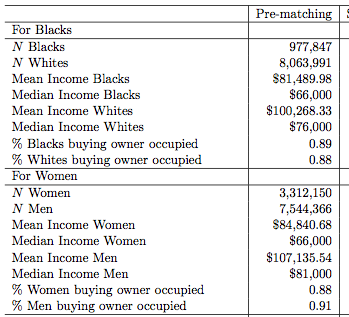
\includegraphics[width = .8 \linewidth]{images/sen.png}
%%\end{figure}
%%
%%\end{frame}
%
%\subsection{Matching}\label{matching}
%
%\begin{frame}{}
%
%\centering
%
%\fbox{Matching is Not an Identification Strategy}
%
%\end{frame}
%
%%\begin{frame}{Lyall (2009)}
%%
%%\begin{figure}[ht] \centering
%%    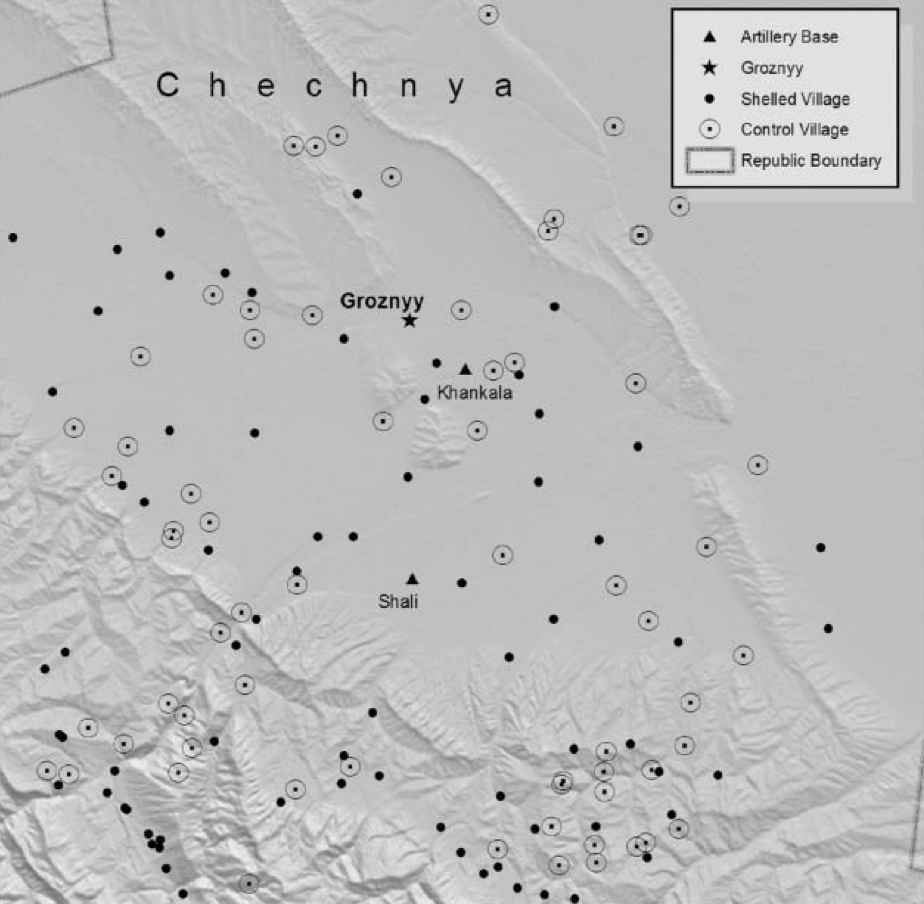
\includegraphics[width = .8 \linewidth]{images/lyall_map.png}
%%\end{figure}
%%
%%\end{frame}
%%
%%\begin{frame}{Identification Strategy: Doctrine and Drunks}
%%
%%\textbf{``Harassment and Interdiction'' Doctrine}: ``barrages at random
%%intervals and of varying duration on random days'' \pause \bigskip
%%
%%\textbf{Drunks}: ``As one Russian commander put it, solders `get drunk
%%as pigs, lob a few shells, claim combat pay and get drunk again'.''"
%%
%%\end{frame}
%%
%%\begin{frame}{Balance Checks}
%%
%%\begin{figure}[ht] \centering
%%    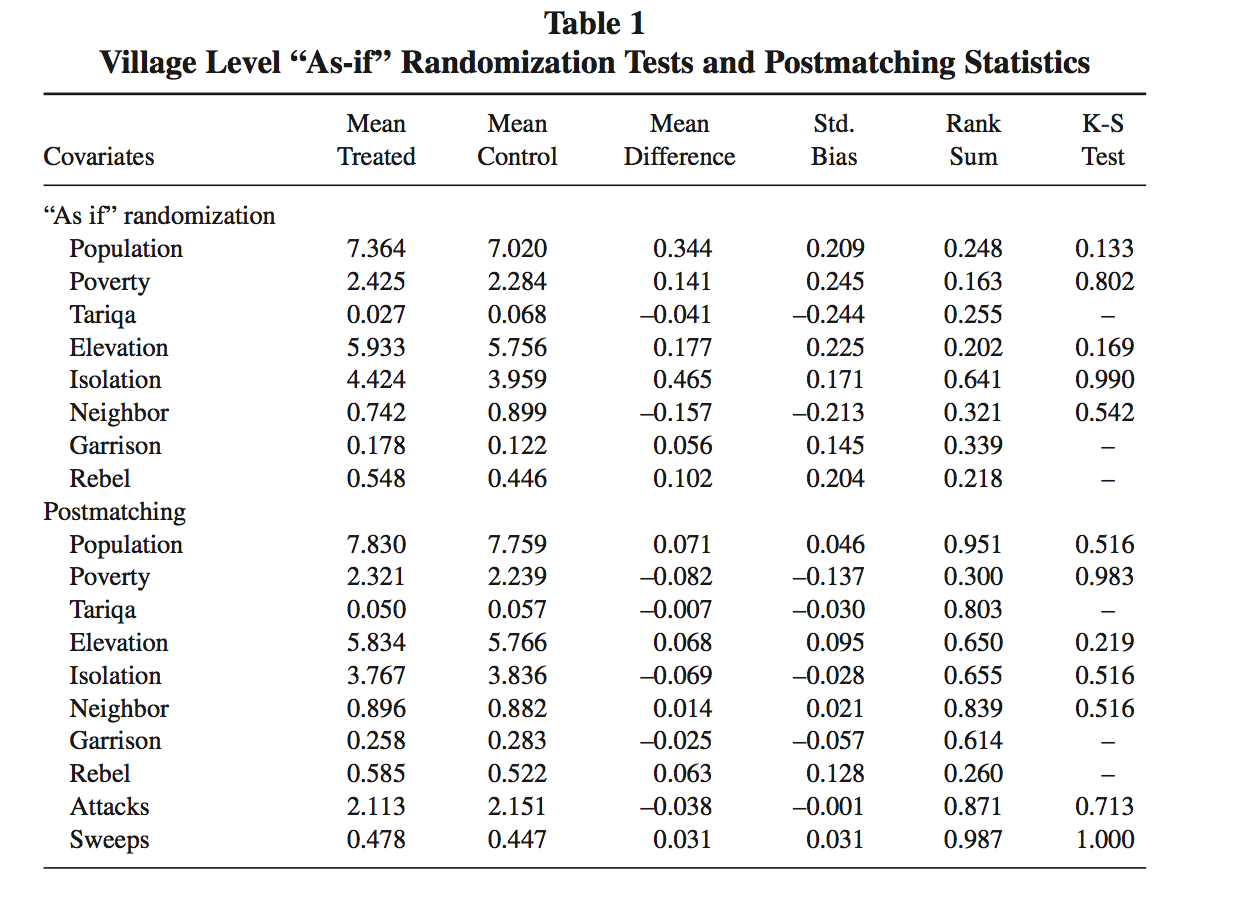
\includegraphics[width = .99 \linewidth]{images/lyall_balance.png}
%%\end{figure}
%%
%%\end{frame}
%
%%\begin{frame}{Gilligan and Sargenti (2008)}
%%
%%\begin{figure}[ht] \centering
%%    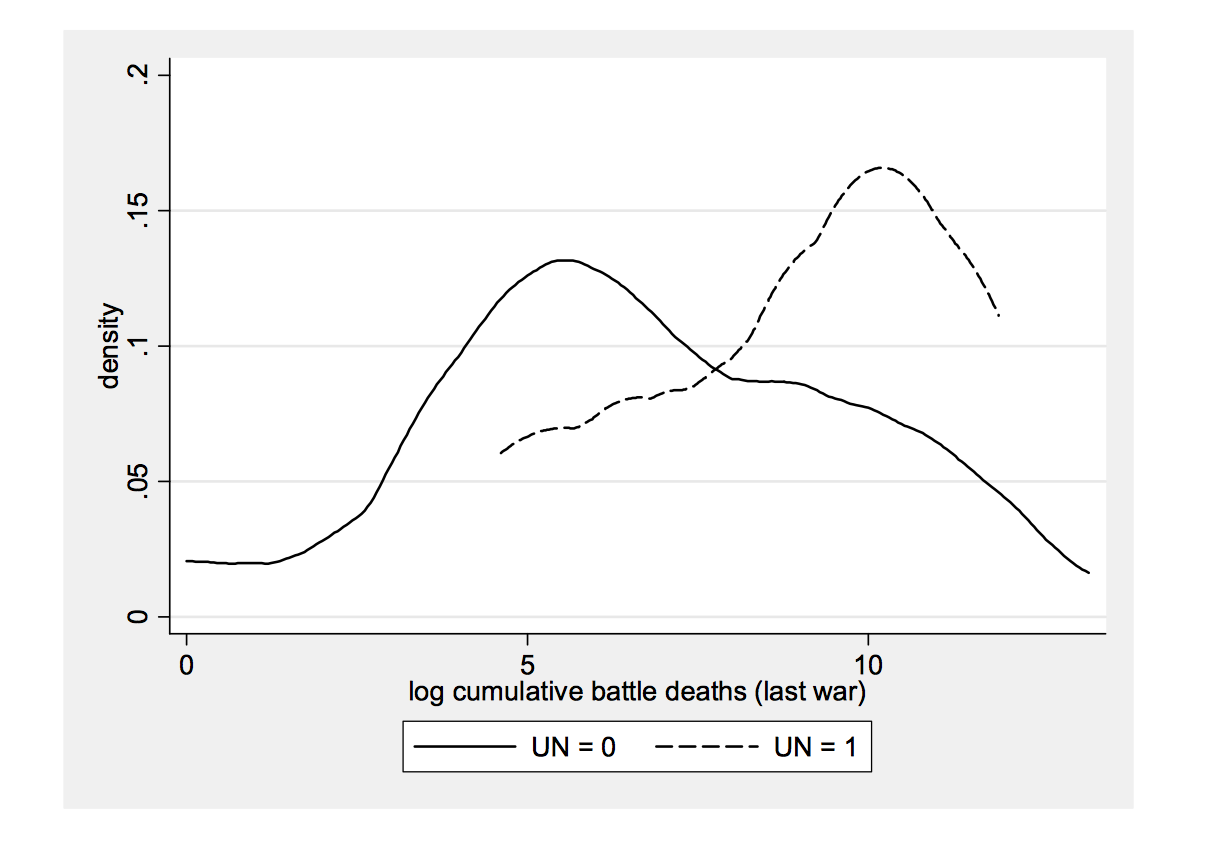
\includegraphics[width = .99 \linewidth]{images/gilligan_sargenti_balance.png}
%%\end{figure}
%%
%%\end{frame}
%
%%\begin{frame}{Gilligan and Sargenti (2008)}
%%
%%\begin{figure}[ht] \centering
%%    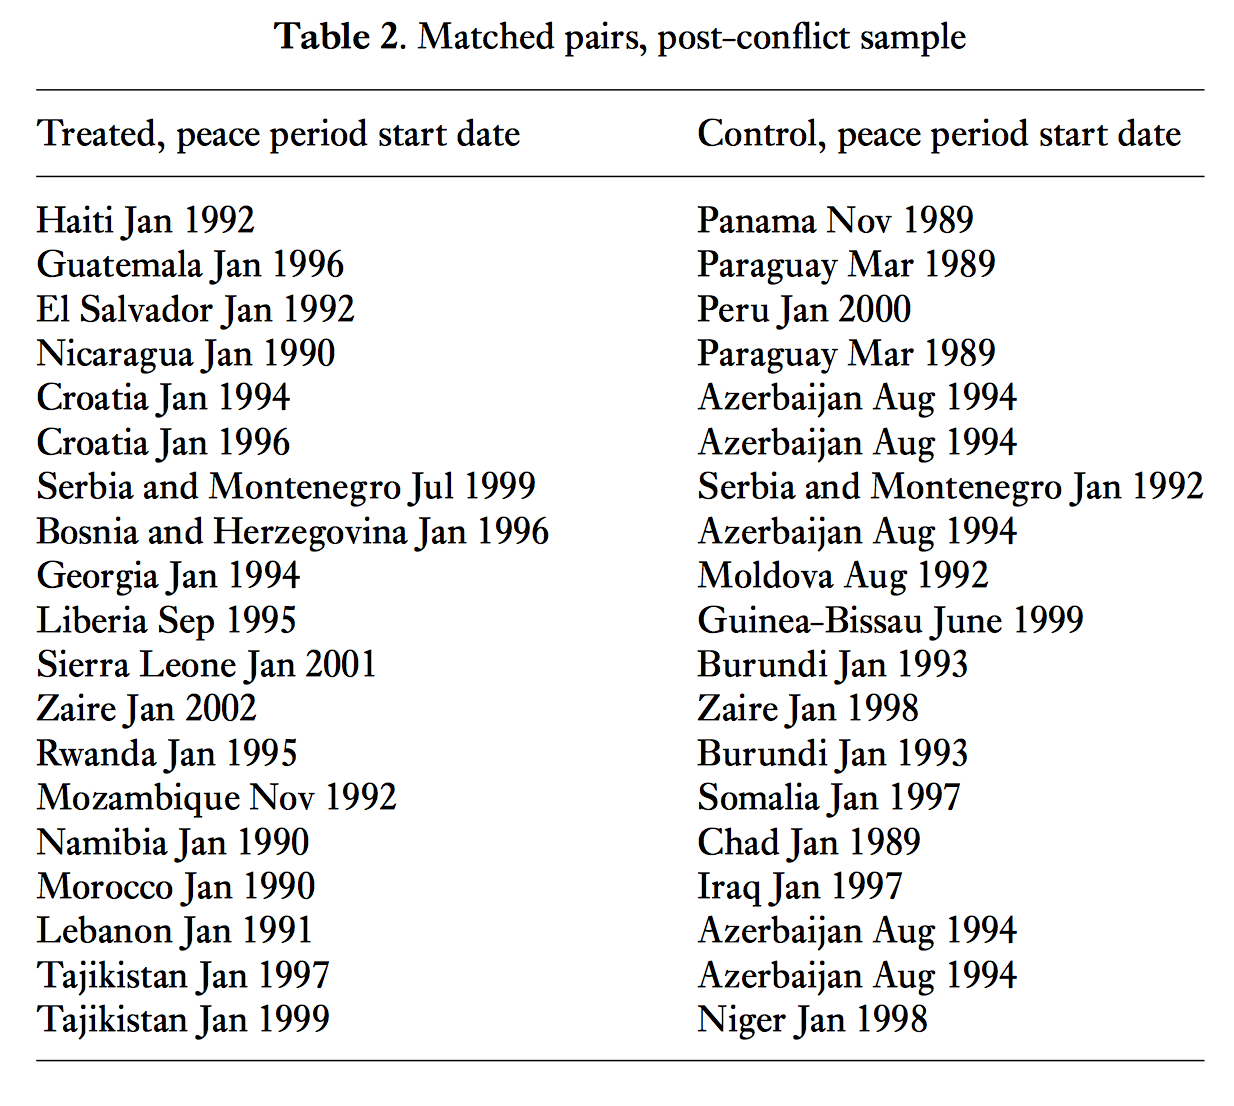
\includegraphics[width = .99 \linewidth]{images/gilligan_sargenti_matched_pairs.png}
%%\end{figure}
%%
%%\end{frame}
%
%
%
%\begin{frame}{Matching}
%
%When $X$ is continuous we can estimate $\tau_{ATT}$ by ``imputing''
%the missing potential outcome of each treated unit using the observed
%outcome from the ``closest'' control unit: \[
%\widehat{\tau}_{ATT}= \frac{1}{N_1} \sum_{D_i=1}
%\big(Y_i - Y_{j(i)}\big)
%\] where $Y_{j(i)}$ is the outcome of an untreated observation such that
%$X_{j(i)}$ is the \alert{closest} value to $X_i$ among the untreated
%observations. \pause
%
%We can also use the average for $M$ closest matches: \[
%\widehat{\tau}_{ATT}= \frac{1}{N_1} \sum_{D_i=1} \left\{ Y_i -
%\left(\frac{1}{M}\sum_{m=1}^M Y_{j_m(i)},\right)\right\}
%\] Works well when we can find good matches for each treated unit
%
%\end{frame}
%
%\begin{frame}{Matching: Example with a Single $X$}
%
%\begin{tabular}{c|c|c|c|c}
% &Potential Outcome & Potential Outcome &   & \\
%unit &under Treatment  & under Control &   &  \\
%
%\hline
%   i  & $Y_{1i}$  & $Y_{0i}$ &    $D_i$ &  $X_i$ \\
%\hline
%         1 & \multicolumn{ 1}{c|}{6} & \multicolumn{ 1}{c|}{\textcolor{red}{?}} &                    1 &          3 \\
%         2 & \multicolumn{ 1}{c|}{1} & \multicolumn{ 1}{c|}{\textcolor{red}{?}} &                    1 &          1 \\
%         3 & \multicolumn{ 1}{c|}{0} & \multicolumn{ 1}{c|}{\textcolor{red}{?}} &                    1 &          10 \\
%\hline
%         4 & \multicolumn{ 1}{c|}{} & \multicolumn{1}{c|}{0} &                    0 &          2 \\
%         5 & \multicolumn{ 1}{c|}{} & \multicolumn{1}{c|}{9} &                    0 &          3 \\
%         6 & \multicolumn{ 1}{c|}{} & \multicolumn{1}{c|}{1} &                    0 &          -2 \\
%         7 & \multicolumn{ 1}{c|}{} & \multicolumn{1}{c|}{1} &                    0 &          -4 \\
%         \hline
%\end{tabular}
%
%What is
%$\widehat{\tau}_{ATT}= \frac{1}{N_1} \sum_{D_i=1} \big(Y_i - Y_{j(i)}\big)$?
%\pause
%
%Match and plugin in
%
%\end{frame}
%
%\begin{frame}{Matching: Example with a Single $X$}
%
%\begin{tabular}{c|c|c|c|c}
% &Potential Outcome & Potential Outcome &   & \\
%unit &under Treatment  & under Control &   &  \\
%
%\hline
%   i  & $Y_{1i}$  & $Y_{0i}$ &    $D_i$ &  $X_i$ \\
%\hline
%         1 & \multicolumn{ 1}{c|}{6} & \multicolumn{ 1}{c|}{\textcolor{blue}{9}} &                    1 &          \textcolor{blue}{3} \\
%         2 & \multicolumn{ 1}{c|}{1} & \multicolumn{ 1}{c|}{\textcolor{cyan}{0}} &                    1 &          \textcolor{cyan}{1} \\
%         3 & \multicolumn{ 1}{c|}{0} & \multicolumn{ 1}{c|}{\textcolor{blue}{9}} &                    1 &          \textcolor{blue}{10} \\
%\hline
%         4 & \multicolumn{ 1}{c|}{} & \multicolumn{1}{c|}{\textcolor{cyan}{0}} &                    0 &          \textcolor{cyan}{2} \\
%         5 & \multicolumn{ 1}{c|}{} & \multicolumn{1}{c|}{\textcolor{blue}{9}} &                    0 &          \textcolor{blue}{3} \\
%         6 & \multicolumn{ 1}{c|}{} & \multicolumn{1}{c|}{1} &                    0 &          -2 \\
%         7 & \multicolumn{ 1}{c|}{} & \multicolumn{1}{c|}{1} &                    0 &          -4 \\
%         \hline
%\end{tabular}
%
%What is
%$\widehat{\tau}_{ATT}= \frac{1}{N_1} \sum_{D_i=1} \big(Y_i - Y_{j(i)}\big)$?
%\pause
%
%$\widehat{\tau}_{ATT}=1/3\cdot(6-\textcolor{blue}{9})+1/3\cdot(1-\textcolor{cyan}{0})+1/3\cdot(0-\textcolor{blue}{9})=-3.7$
%
%\end{frame}
%
%\begin{frame}{Matching Distance Metric}
%\scriptsize
%``Closeness'' is often defined by a \alert{distance metric}. Let
%$X_i=(X_B,X_B,...,X_{ik})'$ and $X_j=(X_{j1},X_{j2},...,X_{jk})'$
%be the covariate vectors for $i$ and $j$.\\\medskip A commonly used distance is
%the \alert{Mahalanobis distance}: \[
%MD(X_i,X_j)=\sqrt{(X_i-X_j)'\Sigma^{-1}(X_i-X_j)}
%\] where $\Sigma$ is the Variance-Covariance-Matrix so the distance metric is scale-invariant and takes into account the correlations. For an exact match
%$MD(X_i,X_j)=0$. 
%
%Other distance metrics can be used, for example Stata's \texttt{nnmatch} by default uses the diagonal matrix of the inverse of the covariate variances (normalized Euclidean distance):
%\[
%StataD(X_i,X_j)=\sqrt{(X_i-X_j)'diag(\Sigma_X^{-1})(X_i-X_j)}
%\]
%
%In \texttt{R}, Genetic matching uses (\texttt{GenMatch(Matching)}): \[
%GeneticD(X_i,X_j) = \sqrt{(X_i - X_j)'(S^{-1/2})'\, W\, S^{-1/2} (X_i - X_j)}
%\] where $W$ is a $(k \times k)$ positive definite weight matrix with
%zeros in off-diagonals.
%
%\end{frame}
%
%%\begin{frame}{Mahalanobis Distance}
%%
%%\begin{figure}[ht] \centering
%%    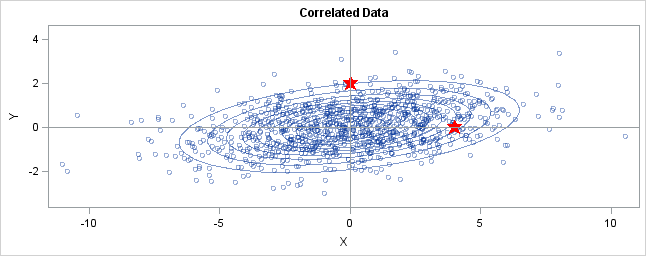
\includegraphics[width = 1 \linewidth]{images/mahal.png}
%%\end{figure}
%%
%%\end{frame}
%%
%%\begin{frame}{Mahalanobis Distance}
%%
%%\begin{figure}[ht] \centering
%%    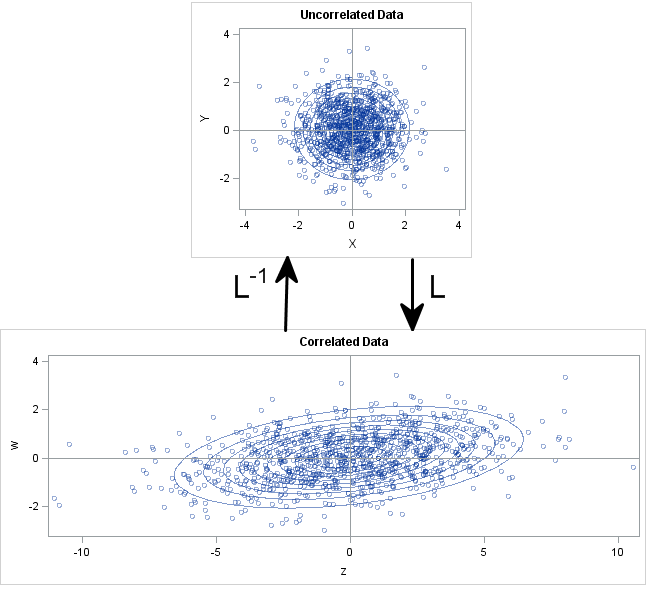
\includegraphics[width = .8 \linewidth]{images/choleskytransform.png}
%%\end{figure}
%%
%%\end{frame}
%
%\begin{frame}{Mahalanobis Distance: Example}
%
%\begin{table}[!h]
% \begin{center}
% \begin{tabular}{ccc}
%\multicolumn{1}{l}{}&
%\multicolumn{1}{c}{$X_1$}&
%\multicolumn{1}{c}{$X_2$}
%\\ \hline
%Treated &$0$&$  0$\\
%Control A &$ 2$&$2$\\
%Control B &$ 1.8$&$0$\\
%\hline
%\end{tabular}
%\end{center}
%\end{table}
%
%$X_T=\left(        \begin{array}{cc}          0 & 0 \\        \end{array}      \right)' $
%$\quad X_A=\left(                 \begin{array}{cc}                   2 & 2 \\                 \end{array}               \right)' $
%$\quad X_B=\left(                 \begin{array}{cc}                   1.8 &  0 \\                 \end{array}               \right)' $\\\bigskip
%
%$\quad\Sigma=\left(                \begin{array}{ccc}                   & X_1 & X_2 \\                  X_1 & 1 &  .9 \\                  X_2 & .9 & 1\\                \end{array}              \right)$\\\bigskip
%
%Which control is closer?
%
%\end{frame}
%
%\begin{frame}{Mahalanobis Distance}
%\scriptsize
%$X_T=\left(        \begin{array}{cc}          0 & 0 \\        \end{array}      \right)' $
%$\,\, X_A=\left(                 \begin{array}{cc}                   2 &  2 \\                 \end{array}               \right)' $
%$\,\, X_B=\left(                 \begin{array}{cc}                   1.8 &  0 \\                 \end{array}               \right)' $
%$\,\,\Sigma=\left(                \begin{array}{ccc}           & X_1 & X_2 \\                  X_1 & 1 &  .9 \\                  X_2 & .9 & 1\\                \end{array}              \right)$
%
%\begin{align*}
%MD(X_A,X_{T}) &= \sqrt{
%(X_A-X_T)'\Sigma^{-1}(X_A-X_T)}\\
% &=  \sqrt{
%(\left(
%       \begin{array}{cc}
%         2 & 2 \\
%       \end{array}
%     \right)-\left(
%                \begin{array}{cc}
%                  0 &  0 \\
%                \end{array}
%              \right))' \left(
%               \begin{array}{cc}
%                  1 &  .9 \\
%                   .9 & 1 \\
%               \end{array}
%             \right)^{-1} (\left(
%       \begin{array}{cc}
%         2 & 2 \\
%       \end{array}
%     \right)-\left(
%                \begin{array}{cc}
%                    0 &  0 \\
%                \end{array}
%              \right))}\\
%& =  \sqrt{
%\left(
%       \begin{array}{cc}
%         2 &  2 \\
%       \end{array}
%     \right)' \left(
%               \begin{array}{cc}
%                   5.2 &  -4.7 \\
%                   -4.7 & 5.2 \\
%               \end{array}
%             \right)\left(
%       \begin{array}{cc}
%         2 &  2 \\
%       \end{array}
%     \right)}\\
% &= 4.2\\
%MD(X_B,X_{T}) &=  \sqrt{
%\left(
%       \begin{array}{cc}
%         1.8 &  0 \\
%       \end{array}
%     \right)' \left(
%               \begin{array}{cc}
%                   5.2 &  -4.7 \\
%                   -4.7 & 5.2 \\
%               \end{array}
%             \right)\left(
%       \begin{array}{cc}
%          1.8 &  0 \\
%       \end{array}
%     \right)}\\
% &= 17\\
%\end{align*}
%With $StataD(X_A,X_T)=\sqrt{(X_i-X_T)'diag(\Sigma_X^{-1})(X_i-X_T)}$ we find $StataD(X_A,X_T)=84$ and $StataD(X_B,X_T)=17$ since correlation is ignored.
%\end{frame}
%
%\begin{frame}{Mahalanobis Distance}
%\vspace{-.2in}
%\begin{figure}[ht] \centering
%    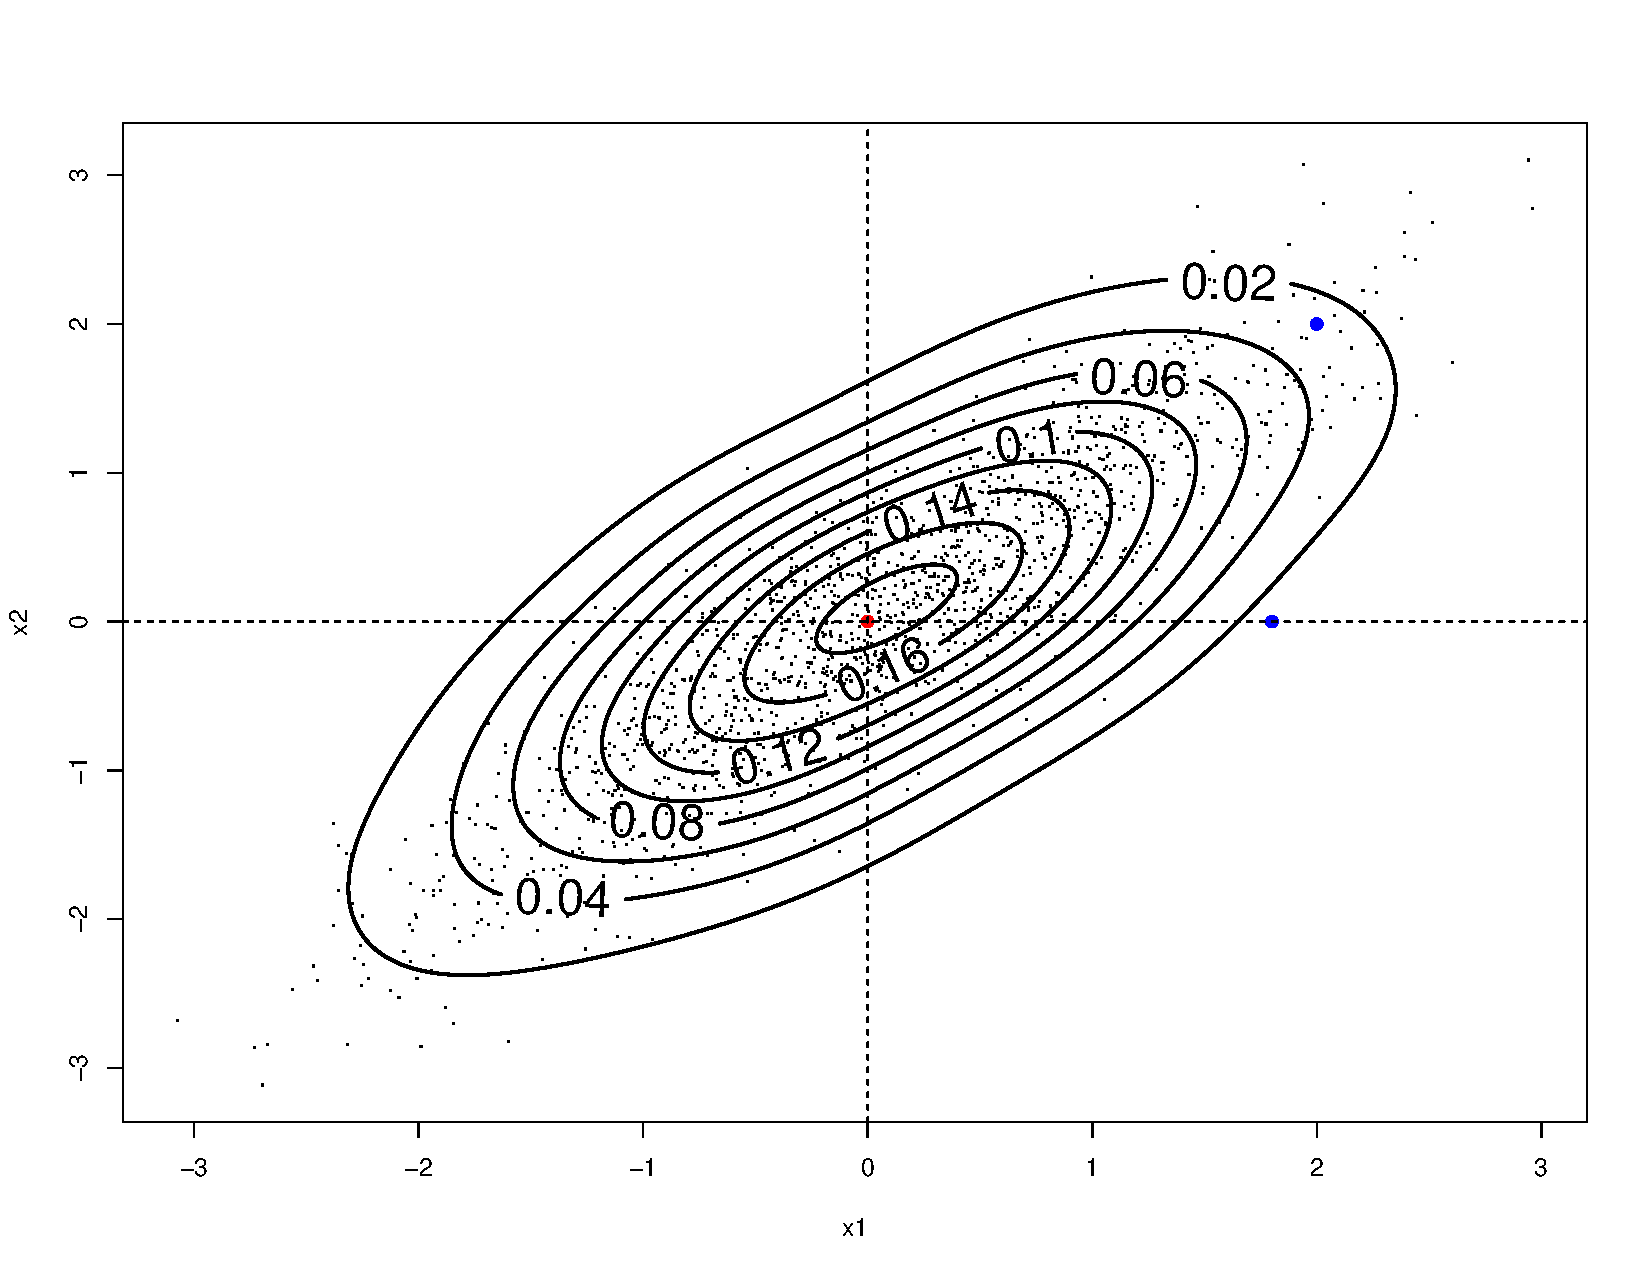
\includegraphics[width = .9 \linewidth]{images/Maha1.pdf}
%\end{figure}
%
%\end{frame}
%
%\begin{frame}{Normalized Euclidean Distance}
%\vspace{-.2in}
%\begin{figure}[ht] \centering
%    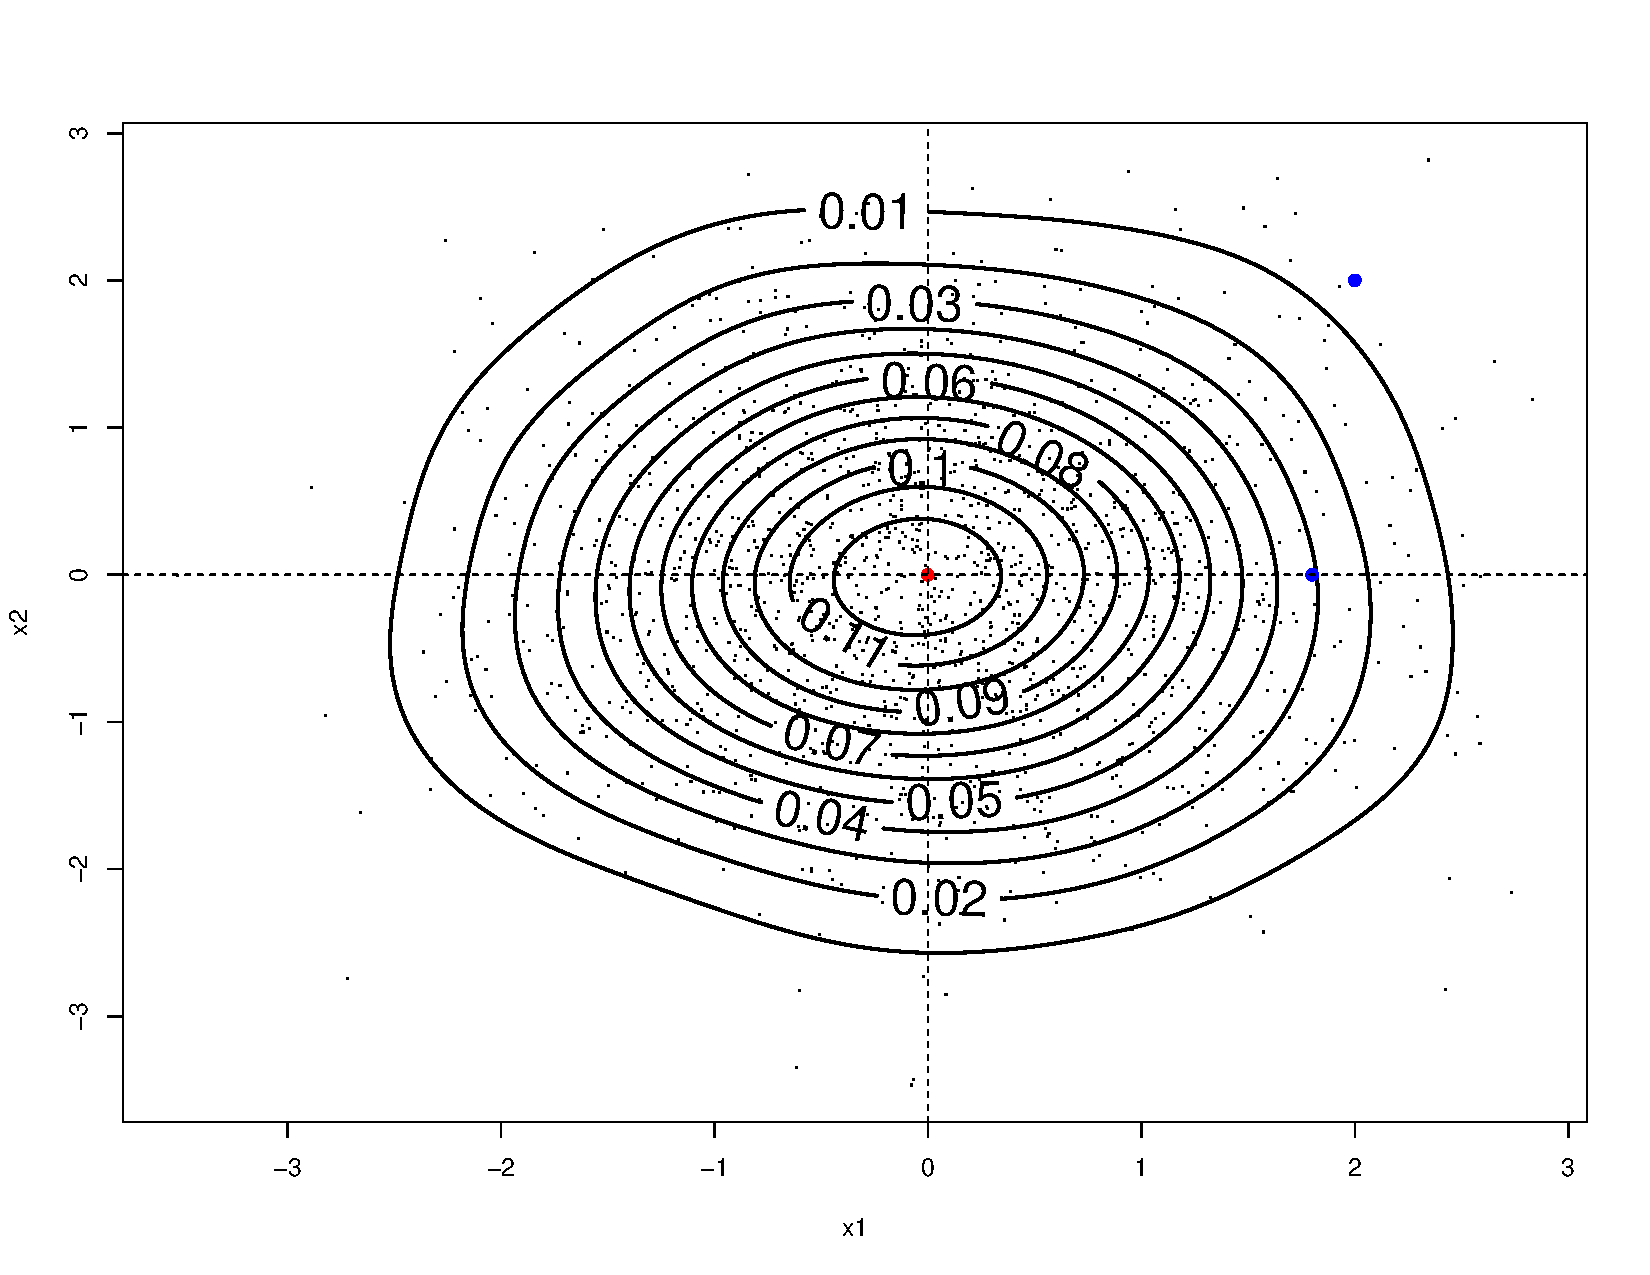
\includegraphics[width = .9 \linewidth]{images/Maha2.pdf}
%\end{figure}
%
%\end{frame}
%
%%\begin{frame}{Genmatch}
%%
%%\begin{figure}[ht] \centering
%%    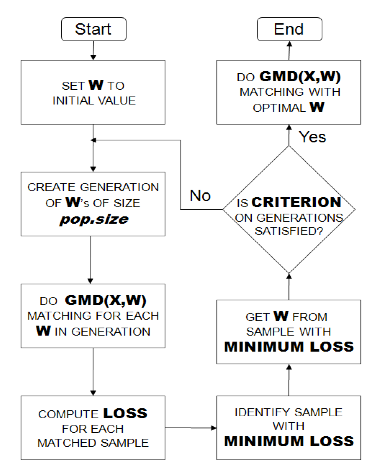
\includegraphics[width = .5 \linewidth]{images/genmatch_flow_chart.png}
%%\end{figure}
%%
%%\end{frame}
%
%%\begin{frame}{Genmatch}
%%
%%\begin{figure}[ht] \centering
%%    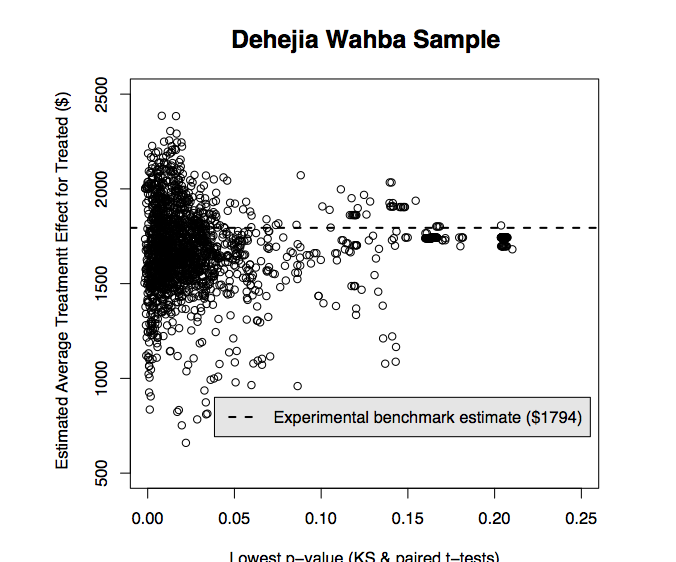
\includegraphics[width = .8 \linewidth]{images/genmatch.png}
%%\end{figure}
%%
%%\end{frame}
%
%\begin{frame}{Local Methods and the Curse of Dimensionality}
%\small
%\textbf{Big} Problem: \pause in a mathematical space, the volume increases \alert{exponentially} when adding extra dimensions.
%\vspace{-.5cm}
%\begin{figure}[ht] \centering
%    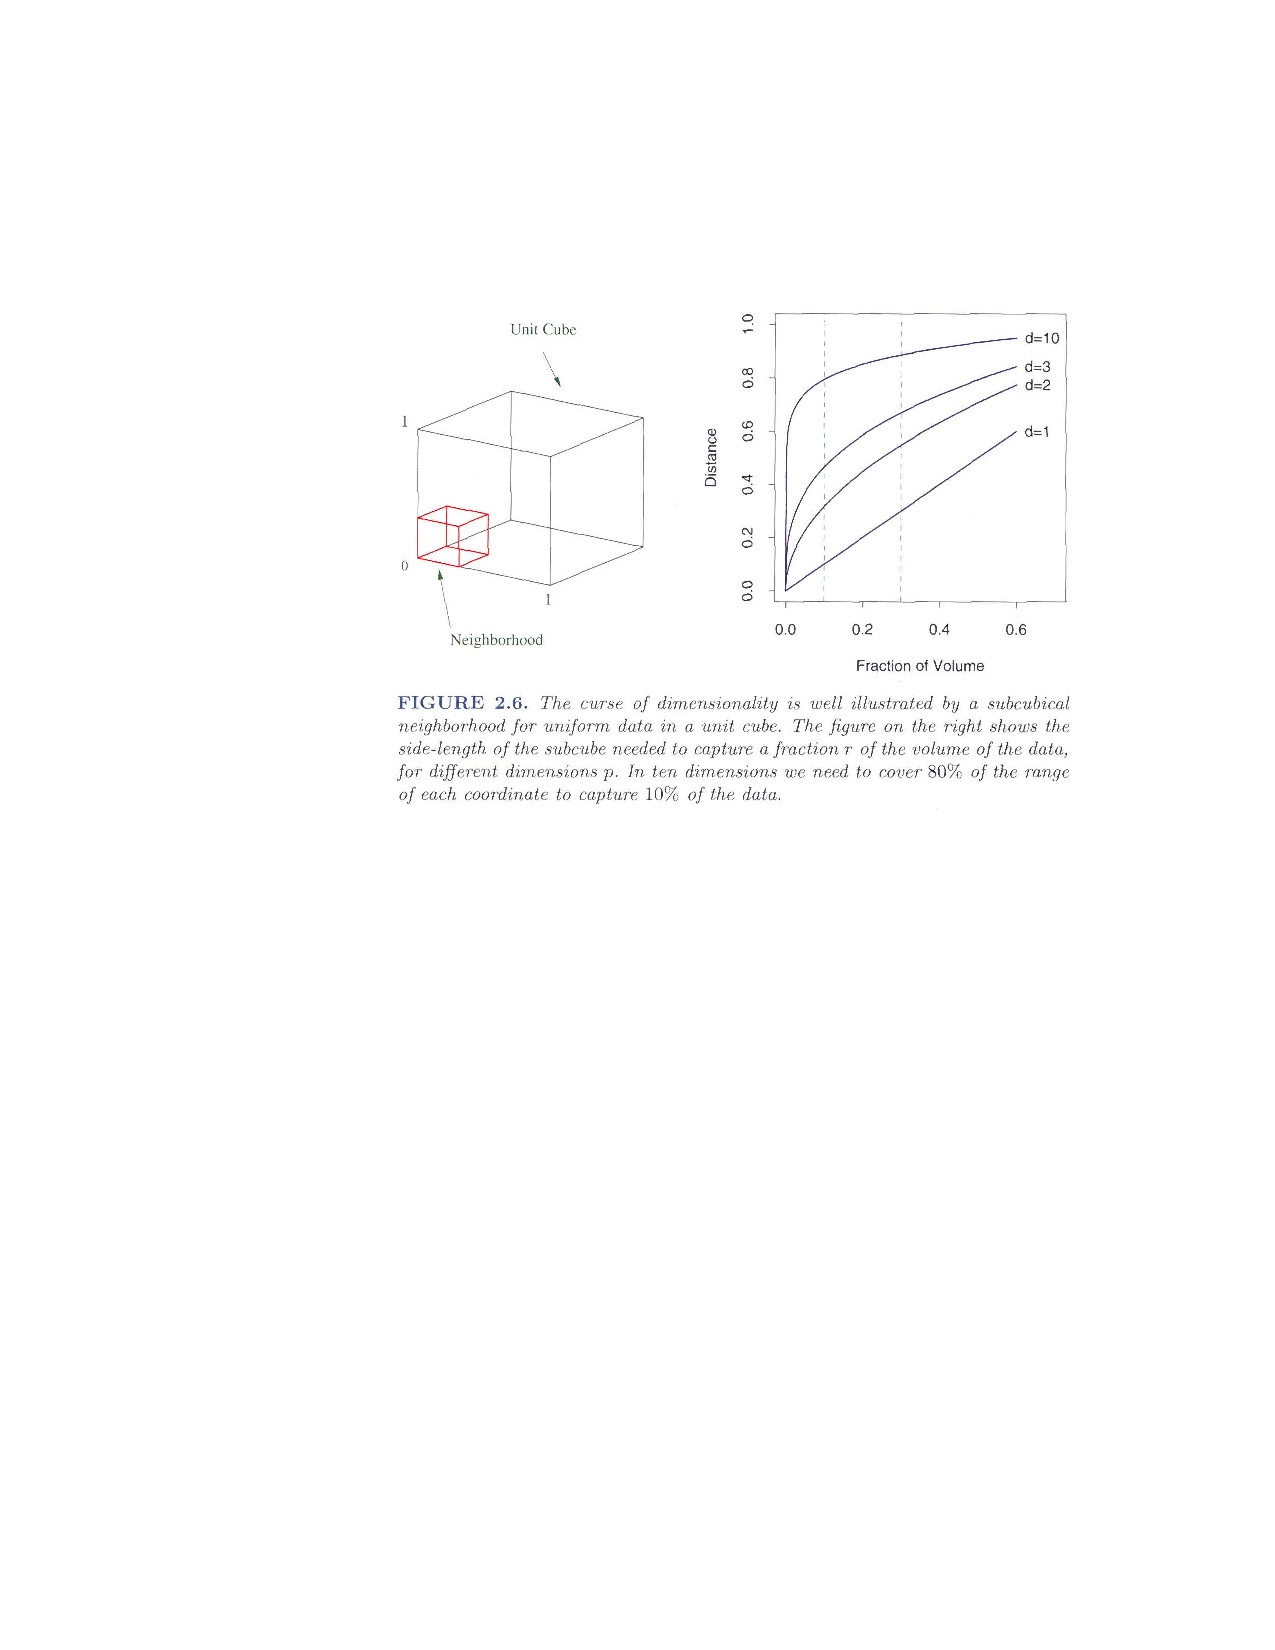
\includegraphics[width = .8 \linewidth]{images/curse_dimensionality1.pdf}
%\end{figure}
%
%\end{frame}
%
%\begin{frame}{Local Methods and the Curse of Dimensionality}
%
%\begin{figure}[ht] \centering
%    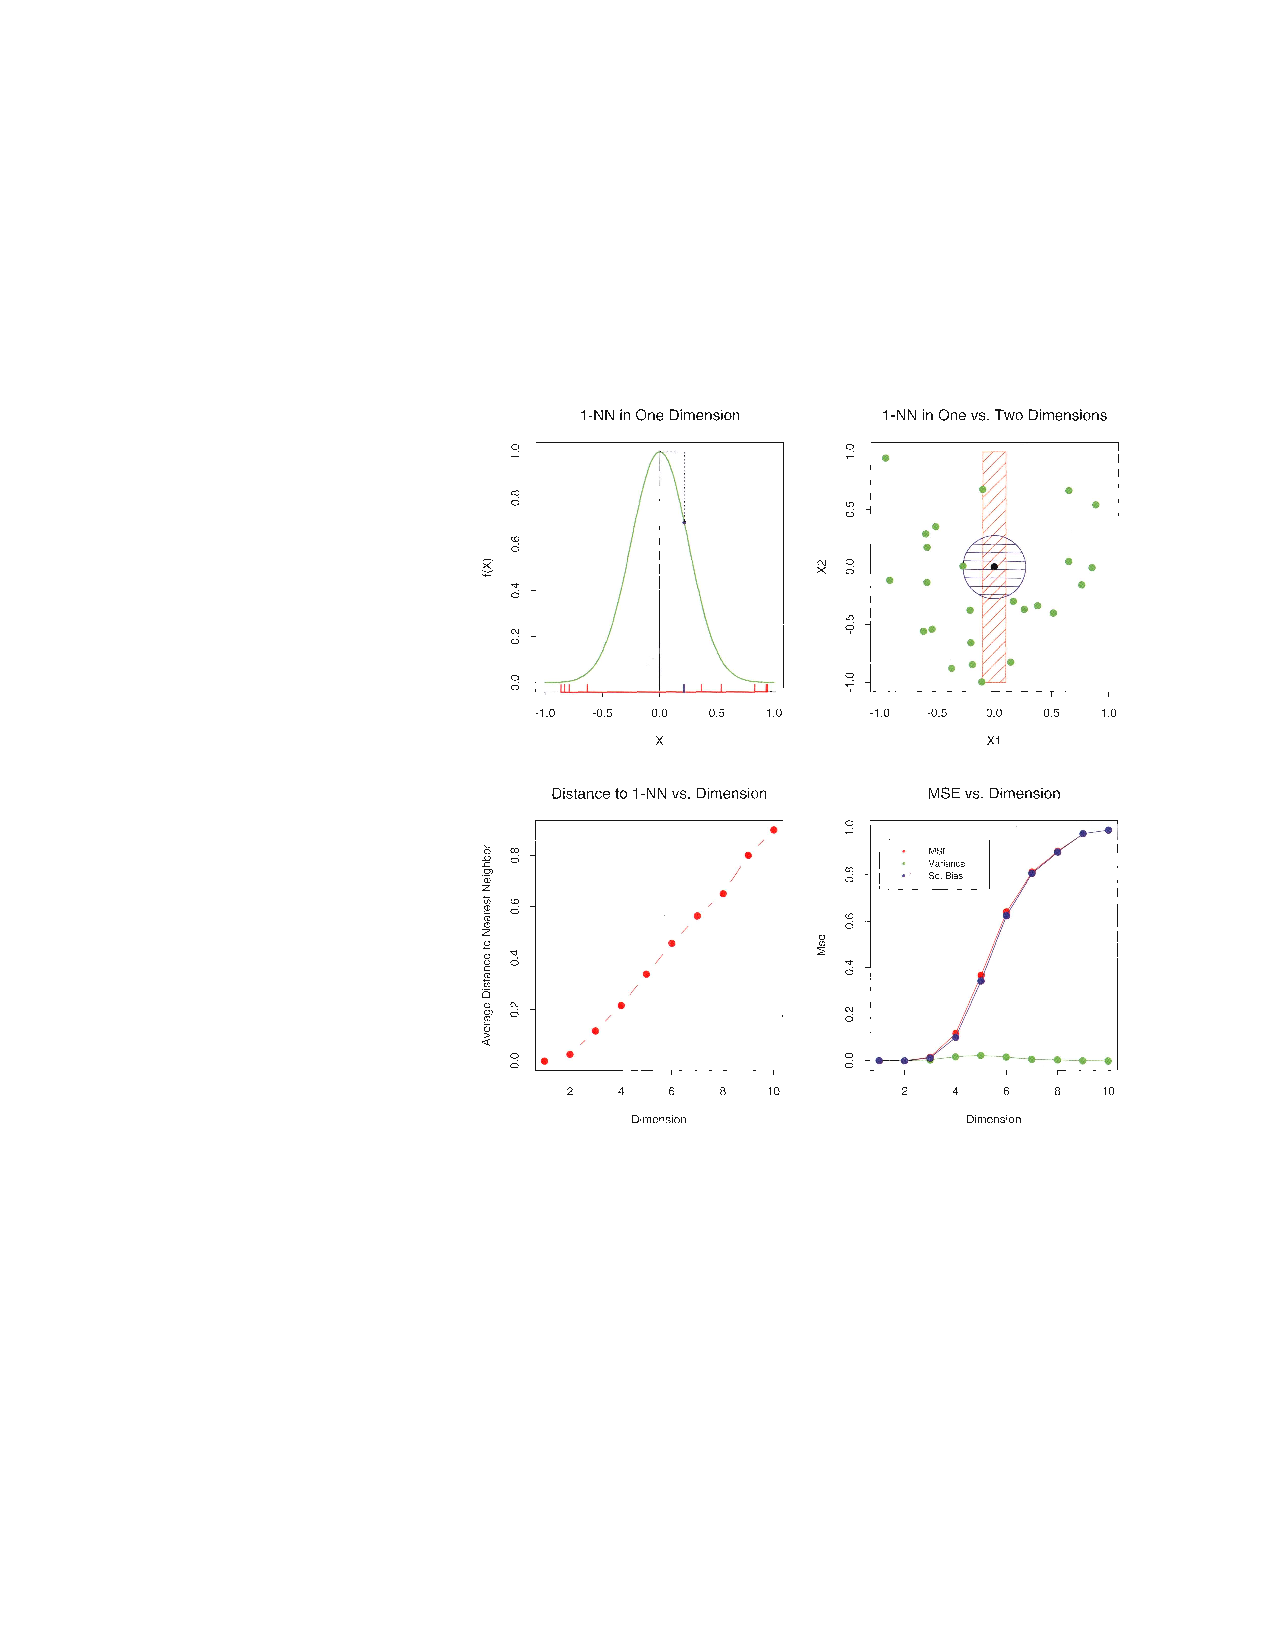
\includegraphics[width = .6 \linewidth]{images/curse_dimensionality2.pdf}
%\end{figure}
%
%\end{frame}
%
%\begin{frame}{Matching with Bias Correction}
%
%Matching estimators may behave badly if $X$ contains multiple continuous
%variables.
%
%Need to adjust matching estimators in the following way: \[
%\tilde{\tau}_{ATT}= \frac{1}{N_1} \sum_{D_i=1}
%(Y_i - Y_{j(i)}) - (\widehat\mu_0(X_i)-\widehat\mu_0(X_{j(i)})),
%\] where $\mu_0(x)=E[Y|X=x, W=0]$ is the population regression function
%under the control condition and $\widehat \mu_0$ is an estimate of
%$\mu_0$.
%
%$X_i-X_{j(i)}$ is often referred to as the \alert{matching discrepancy}.
%
%These ``bias-corrected'' matching estimators behave well even if $\mu_0$
%is estimated using a simple linear regression (ie.
%$\mu_0(x)=\beta_0 + \beta_1 x$) (Abadie and Imbens, 2005)
%
%\end{frame}
%
%\begin{frame}{Matching with Bias Correction}
%
%Each treated observation contributes \[
%\mu_0(X_i)-\mu_0(X_{j(i)})
%\] to the bias.
%
%Bias-corrected matching: \[
%\tilde\tau_{ATT}= \frac{1}{N_1}\sum_{D_i=1} \Big((Y_i-Y_{j(i)})-
%(\widehat\mu_0(X_i)-\widehat\mu_0(X_{j(i)})).
%\Big)
%\] The large sample distribution of this estimator (for the case of
%matching with replacement) is (basically) standard normal. $\mu_0$ is
%usually estimated using a simple linear regression (ie.
%$\mu_0(x)=\beta_0 + \beta_1 x$).\\\bigskip
%
%In R: \texttt{Match(Y,Tr, X,BiasAdjust = TRUE)}
%
%\end{frame}
%
%\begin{frame}{Bias Adjustment with Matched Data}
%
%\begin{tabular}{c|c|c|c|c}
% &Potential Outcome & Potential Outcome &   & \\
%unit &under Treatment  & under Control &   &  \\
%
%\hline
%   i  & $Y_{1i}$  & $Y_{0i}$ &    $D_i$ &  $X_i$ \\
%\hline
%         1 & \multicolumn{ 1}{c|}{6} & \multicolumn{ 1}{c|}{\textcolor{red}{?}} &                    1 &          3 \\
%         2 & \multicolumn{ 1}{c|}{1} & \multicolumn{ 1}{c|}{\textcolor{red}{?}} &                    1 &          1 \\
%         3 & \multicolumn{ 1}{c|}{0} & \multicolumn{ 1}{c|}{\textcolor{red}{?}} &                    1 &          10 \\
%\hline
%         4 & \multicolumn{ 1}{c|}{} & \multicolumn{1}{c|}{0} &                    0 &          2 \\
%         5 & \multicolumn{ 1}{c|}{} & \multicolumn{1}{c|}{9} &                    0 &          3 \\
%         6 & \multicolumn{ 1}{c|}{} & \multicolumn{1}{c|}{1} &                    0 &          8 \\
%         \hline
%\end{tabular}
%
%What is
%$\tilde\tau_{ATT}= \frac{1}{N_1}\sum_{D_i=1} \Big((Y_i-Y_{j(i)})- (\widehat\mu_0(X_i)-\widehat\mu_0(X_{j(i)})) \Big)$?
%
%\end{frame}
%
%\begin{frame}{Bias Adjustment with Matched Data}
%
%\footnotesize 
%
%\begin{tabular}{c|c|c|c|c}
% &Potential Outcome & Potential Outcome &   & \\
%unit &under Treatment  & under Control &   &  \\
%\hline
%   i  & $Y_{1i}$  & $Y_{0i}$ &    $D_i$ &  $X_i$ \\
%\hline
%         1 & \multicolumn{ 1}{c|}{6} & \multicolumn{ 1}{c|}{\textcolor{blue}{9}} &                    1 &          3 \\
%         2 & \multicolumn{ 1}{c|}{1} & \multicolumn{ 1}{c|}{\textcolor{cyan}{0}} &                    1 &          1 \\
%         3 & \multicolumn{ 1}{c|}{0} & \multicolumn{ 1}{c|}{\textcolor{green}{1}} &                    1 &          10 \\
%\hline
%         4 & \multicolumn{ 1}{c|}{} & \multicolumn{1}{c|}{0} &                    0 &          \textcolor{cyan}{2} \\
%         5 & \multicolumn{ 1}{c|}{} & \multicolumn{1}{c|}{9} &                    0 &          \textcolor{blue}{3} \\
%         6 & \multicolumn{ 1}{c|}{} & \multicolumn{1}{c|}{1} &                    0 &          \textcolor{green}{8} \\
%         \hline
%\end{tabular}
%
%What is
%$\tilde\tau_{ATT}= \frac{1}{N_1}\sum_{D_i=1} \Big((Y_i-Y_{j(i)})- (\widehat\mu_0(X_i)-\widehat\mu_0(X_{j(i)})) \Big)$?
%
%Estimate $\widehat\mu_0(x)=\beta_0 + \beta_1 x = 5 - .4 x$. \pause Now
%plug in:
%
%\begin{eqnarray*}
%\widehat{\tau}_{ATT} &=&1/3 \{ ((6-\textcolor{blue}{9})-(\widehat\mu_0(3)-\widehat\mu_0(\textcolor{blue}{3})))\\
%&+&((1-\textcolor{cyan}{0})-(\widehat\mu_0(1)-\widehat\mu_0(\textcolor{cyan}{2})))\\
%&+&((0-\textcolor{green}{1})-
%(\widehat\mu_0(10)-\widehat\mu_0(\textcolor{green}{8})))\}\\
%&=& -0.86
%\end{eqnarray*}
%
%Unadjusted: \$ 1/3((6-9) + (1-0) + (0-1) )=-1\$
%
%\end{frame}
%
%\begin{frame}{Before Matching}
%\vspace{-.3in}
%\begin{figure}[ht] \centering
%    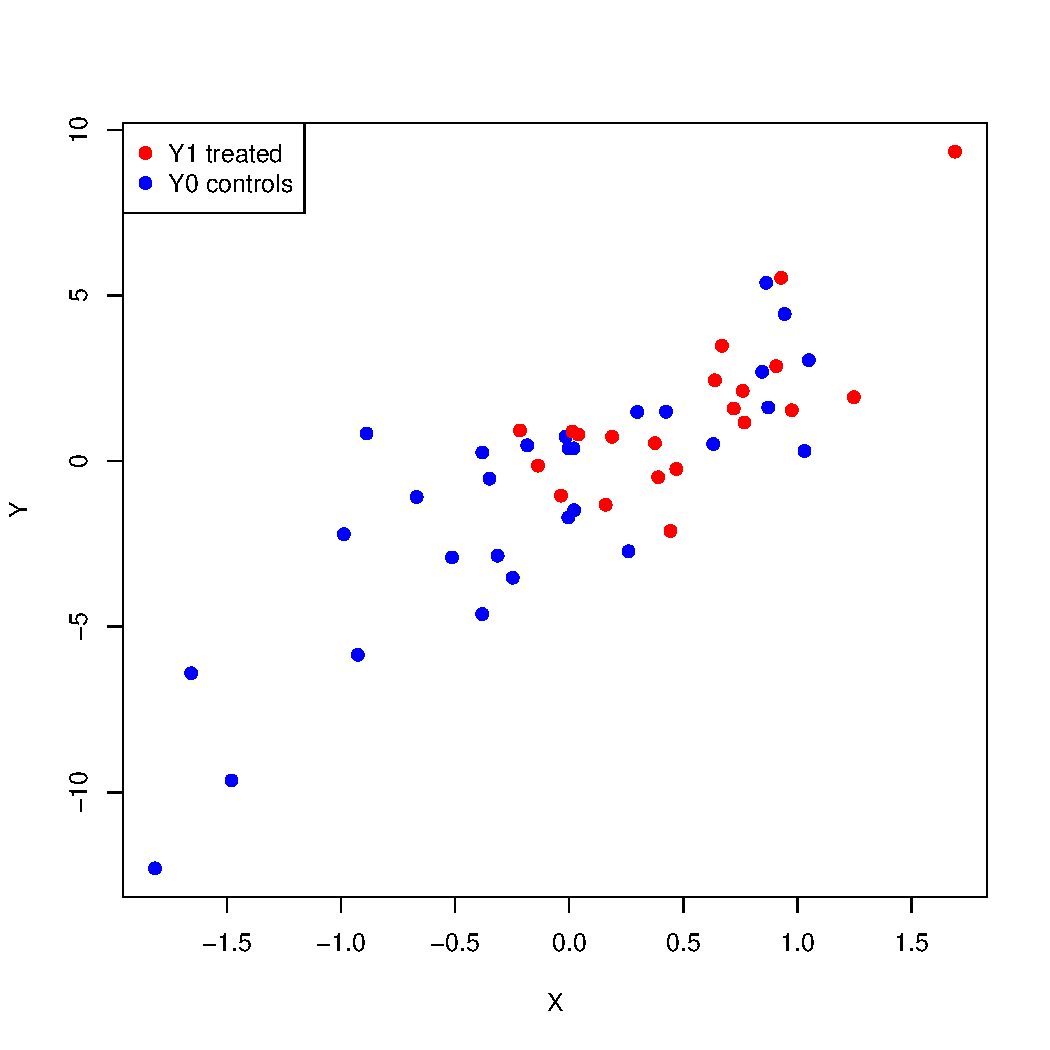
\includegraphics[width = .75 \linewidth]{images/matching_sim1.pdf}
%\end{figure}
%
%\end{frame}
%
%\begin{frame}{After Matching}
%\vspace{-.3in}
%\begin{figure}[ht] \centering
%    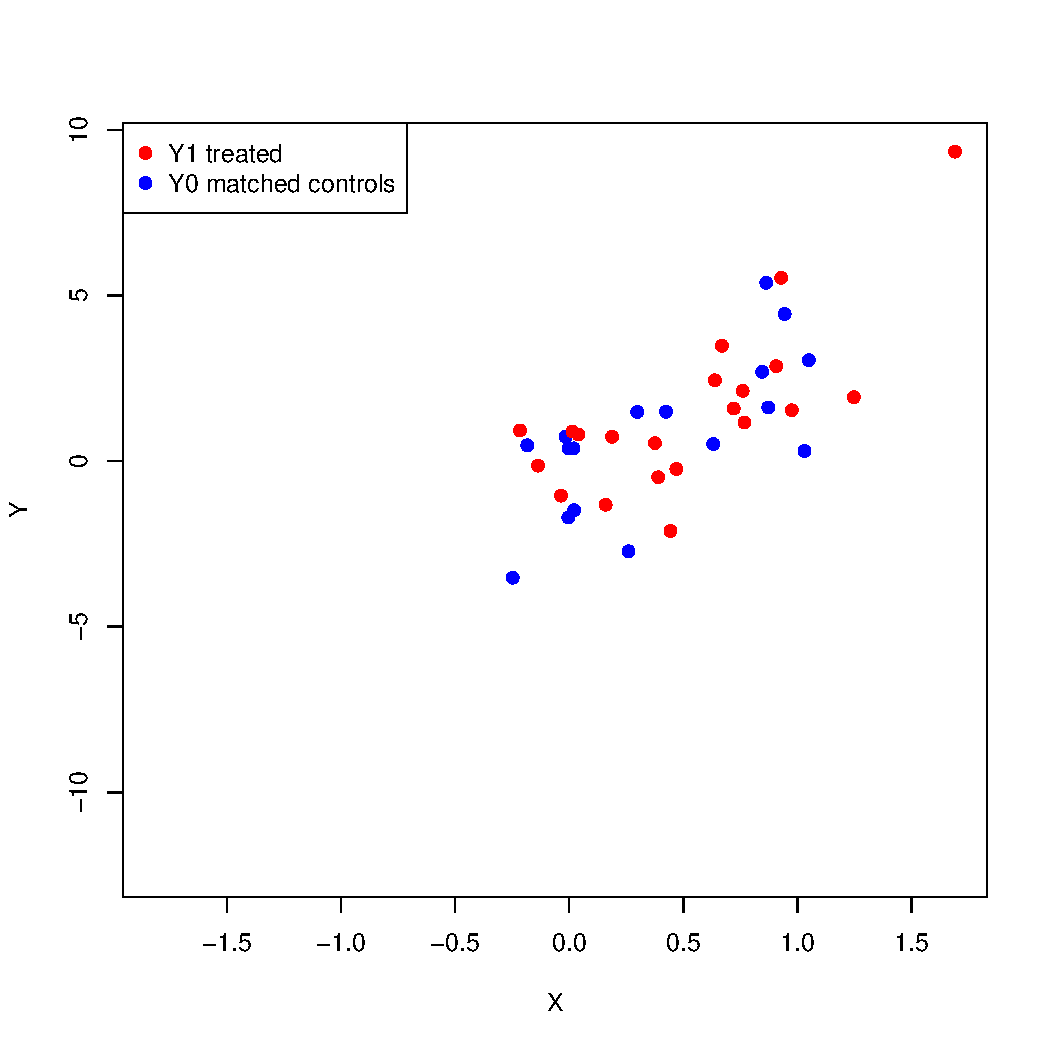
\includegraphics[width = .75 \linewidth]{images/matching_sim2.pdf}
%\end{figure}
%
%\end{frame}
%
%\begin{frame}{After Matching: Imputation Function}
%\vspace{-.3in}
%\begin{figure}[ht] \centering
%    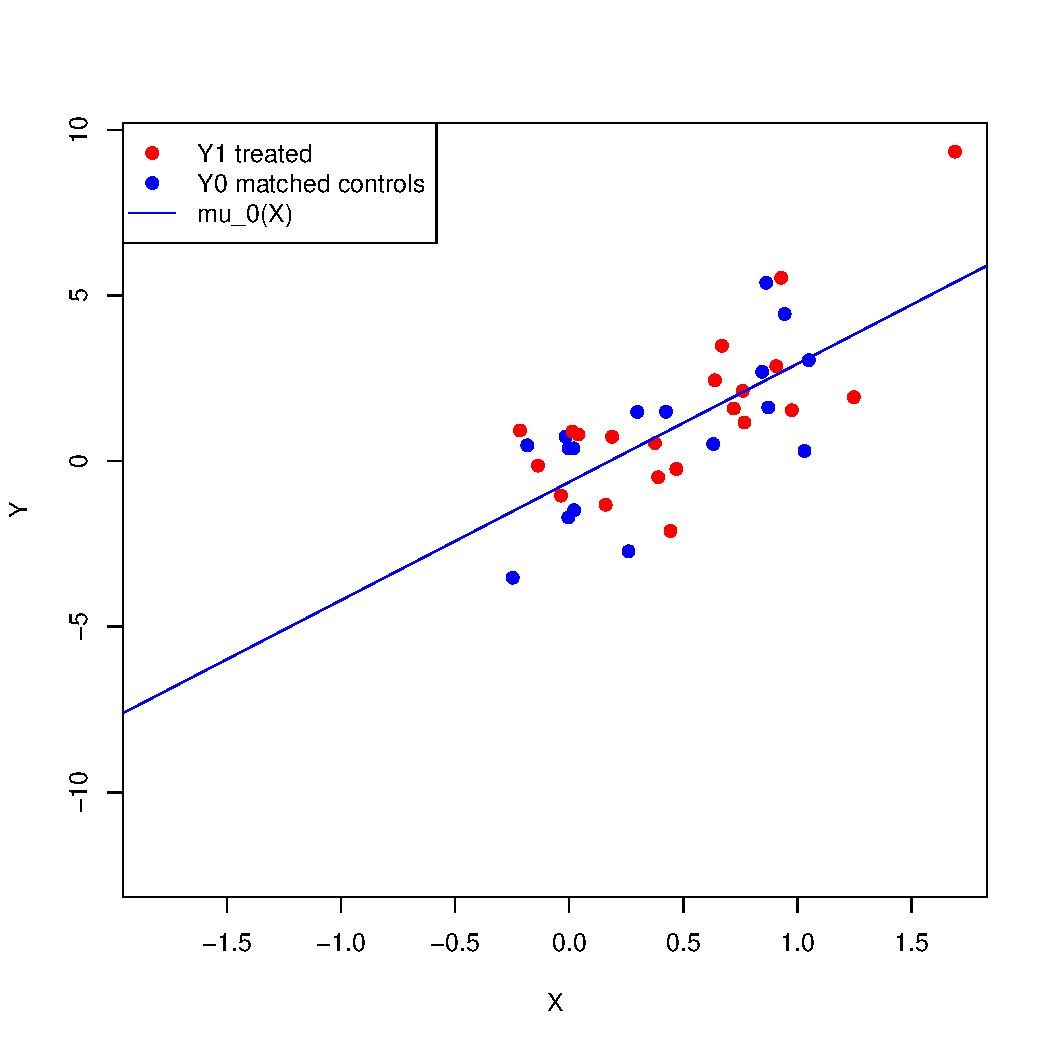
\includegraphics[width = .75 \linewidth]{images/matching_sim3.pdf}
%\end{figure}
%
%\end{frame}
%
%\begin{frame}{After Matching: Imputation of missing $Y_0$}
%\vspace{-.3in}
%\begin{figure}[ht] \centering
%    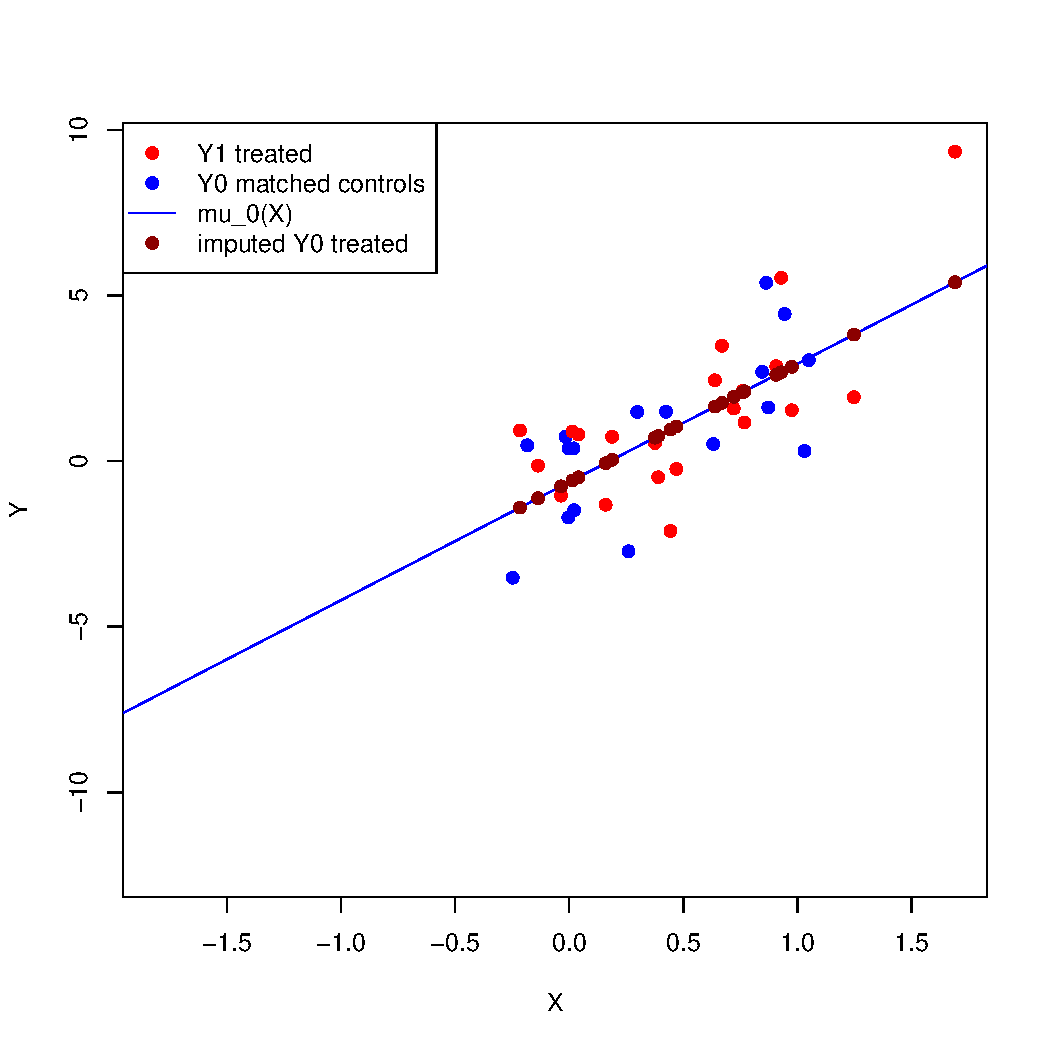
\includegraphics[width = .75 \linewidth]{images/matching_sim4.pdf}
%\end{figure}
%
%\end{frame}
%
%\begin{frame}{After Matching: No Overlap in $Y_0$}
%\vspace{-.3in}
%\begin{figure}[ht] \centering
%    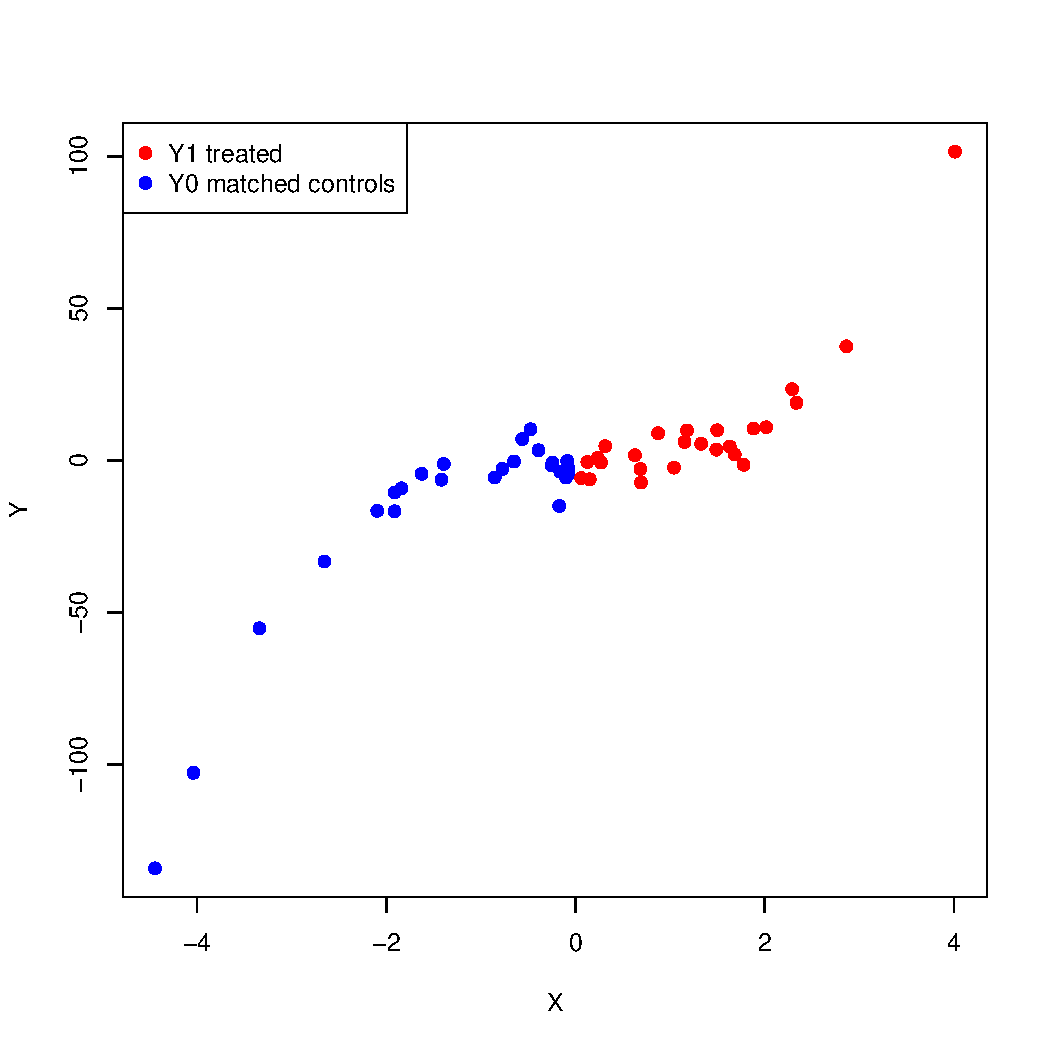
\includegraphics[width = .75 \linewidth]{images/matching_sim5.pdf}
%\end{figure}
%
%\end{frame}
%
%\begin{frame}{After Matching: Imputation of missing $Y_0$}
%\vspace{-.3in}
%\begin{figure}[ht] \centering
%    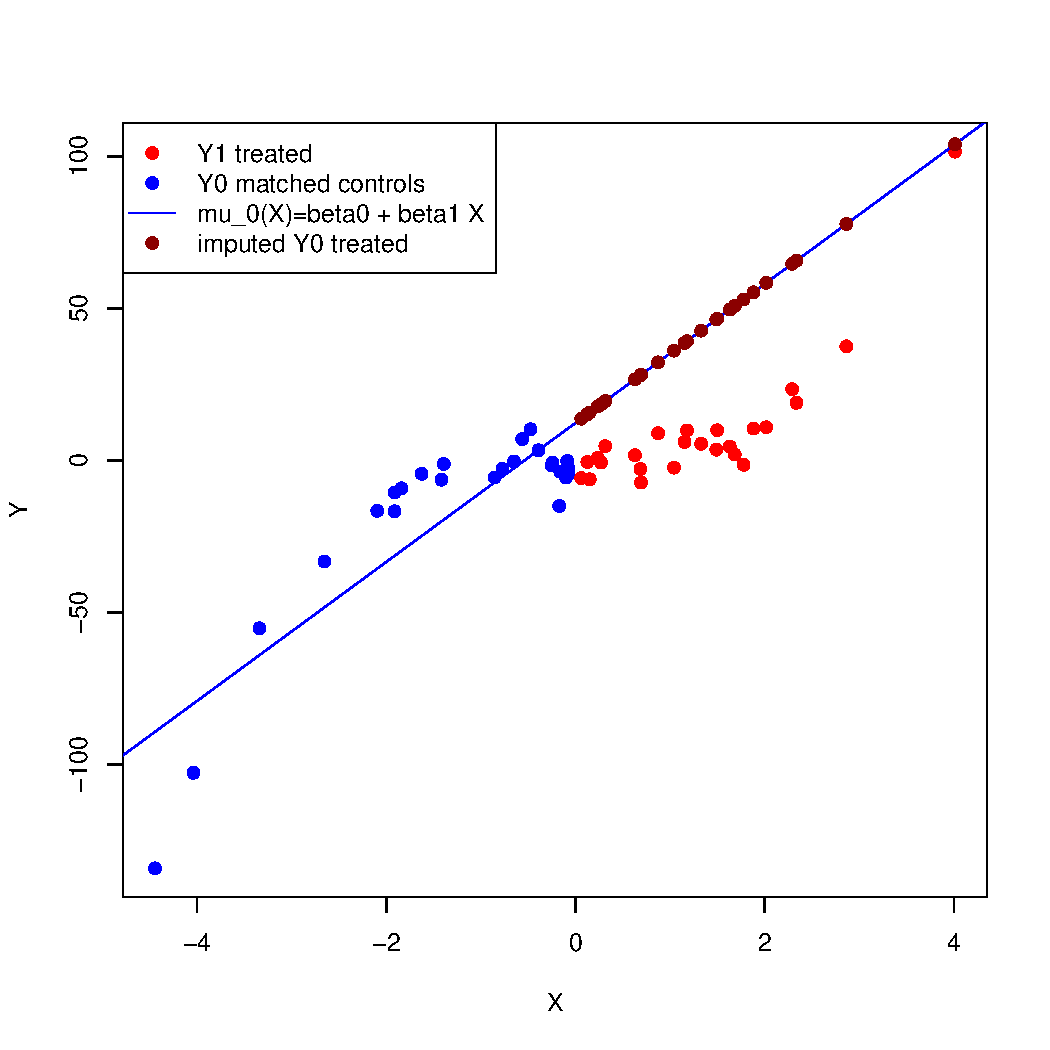
\includegraphics[width = .75 \linewidth]{images/matching_sim6.pdf}
%\end{figure}
%
%\end{frame}
%
%\begin{frame}{After Matching: Imputation of missing $Y_0$}
%\vspace{-.3in}
%\begin{figure}[ht] \centering
%    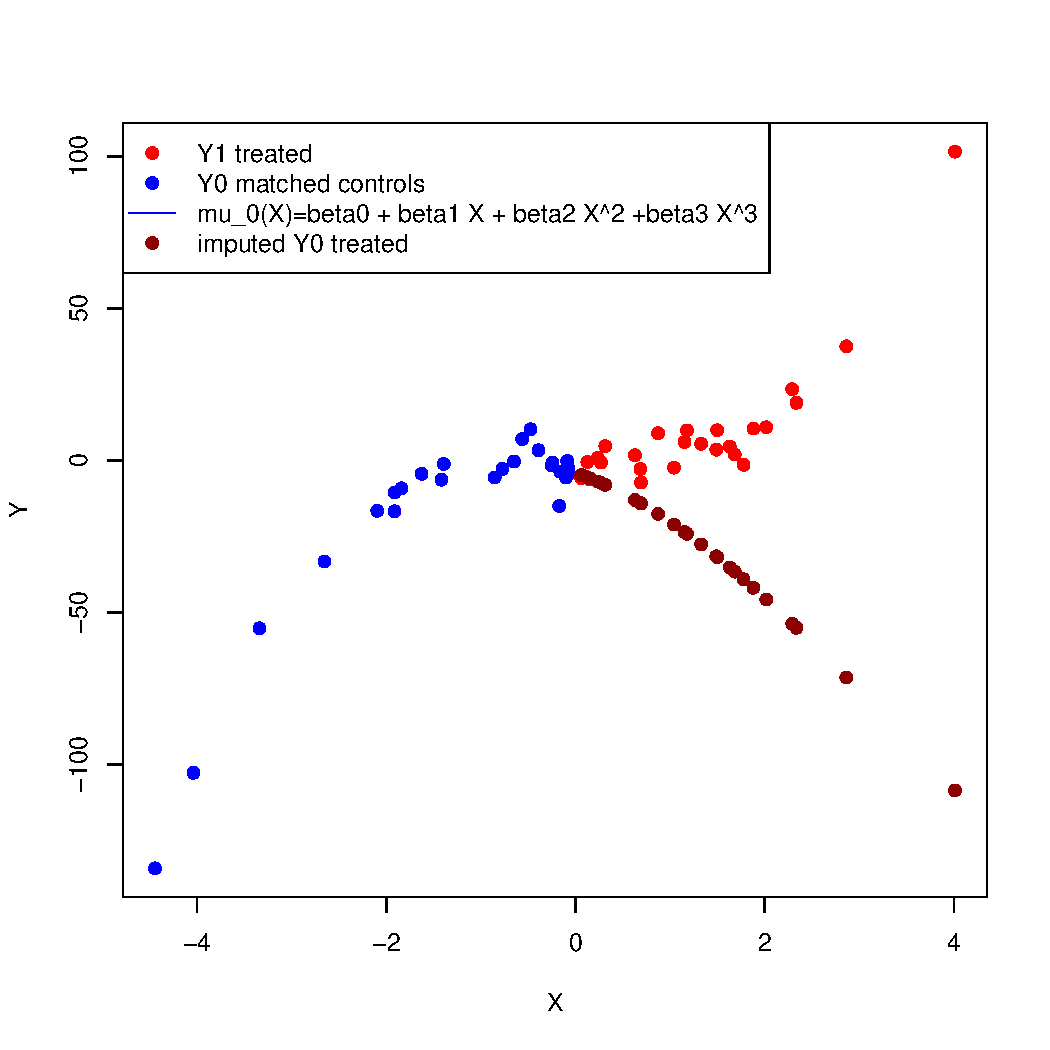
\includegraphics[width = .75 \linewidth]{images/matching_sim7.pdf}
%\end{figure}
%
%\end{frame}
%
%\begin{frame}{Choices when Matching}
%
%\begin{itemize}
%\itemsep1pt\parskip0pt\parsep0pt
%\item
%  With or Without Replacement? \pause
%\item
%  How many matches? \pause
%\item
%  Which Matching Algorithm?
%
%  \begin{itemize}
%  \itemsep1pt\parskip0pt\parsep0pt
%  \item
%    Genetic Matching
%  \item
%    Kernel Matching
%  \item
%    Full Matching
%  \item
%    Coarsened Exact Matching
%  \item
%    Matching as Pre-processing
%  \item
%    Propensity Score Matching \pause
%  \end{itemize}
%\item
%  Use whatever gives you the best balance! Checking balance is important
%  to get a sense for how much extrapolation is needed
%
%  \begin{itemize}
%  \itemsep1pt\parskip0pt\parsep0pt
%  \item
%    Should check balance on interactions and higher moments
%  \end{itemize}
%\item
%  With insufficient overlap, all adjustment methods are problematic
%  because we have to heavily rely on a model to impute missing potential
%  outcomes.
%\end{itemize}
%
%\end{frame}
%
%\begin{frame}{Balance Checks}
%
%\begin{figure}[ht] \centering
%    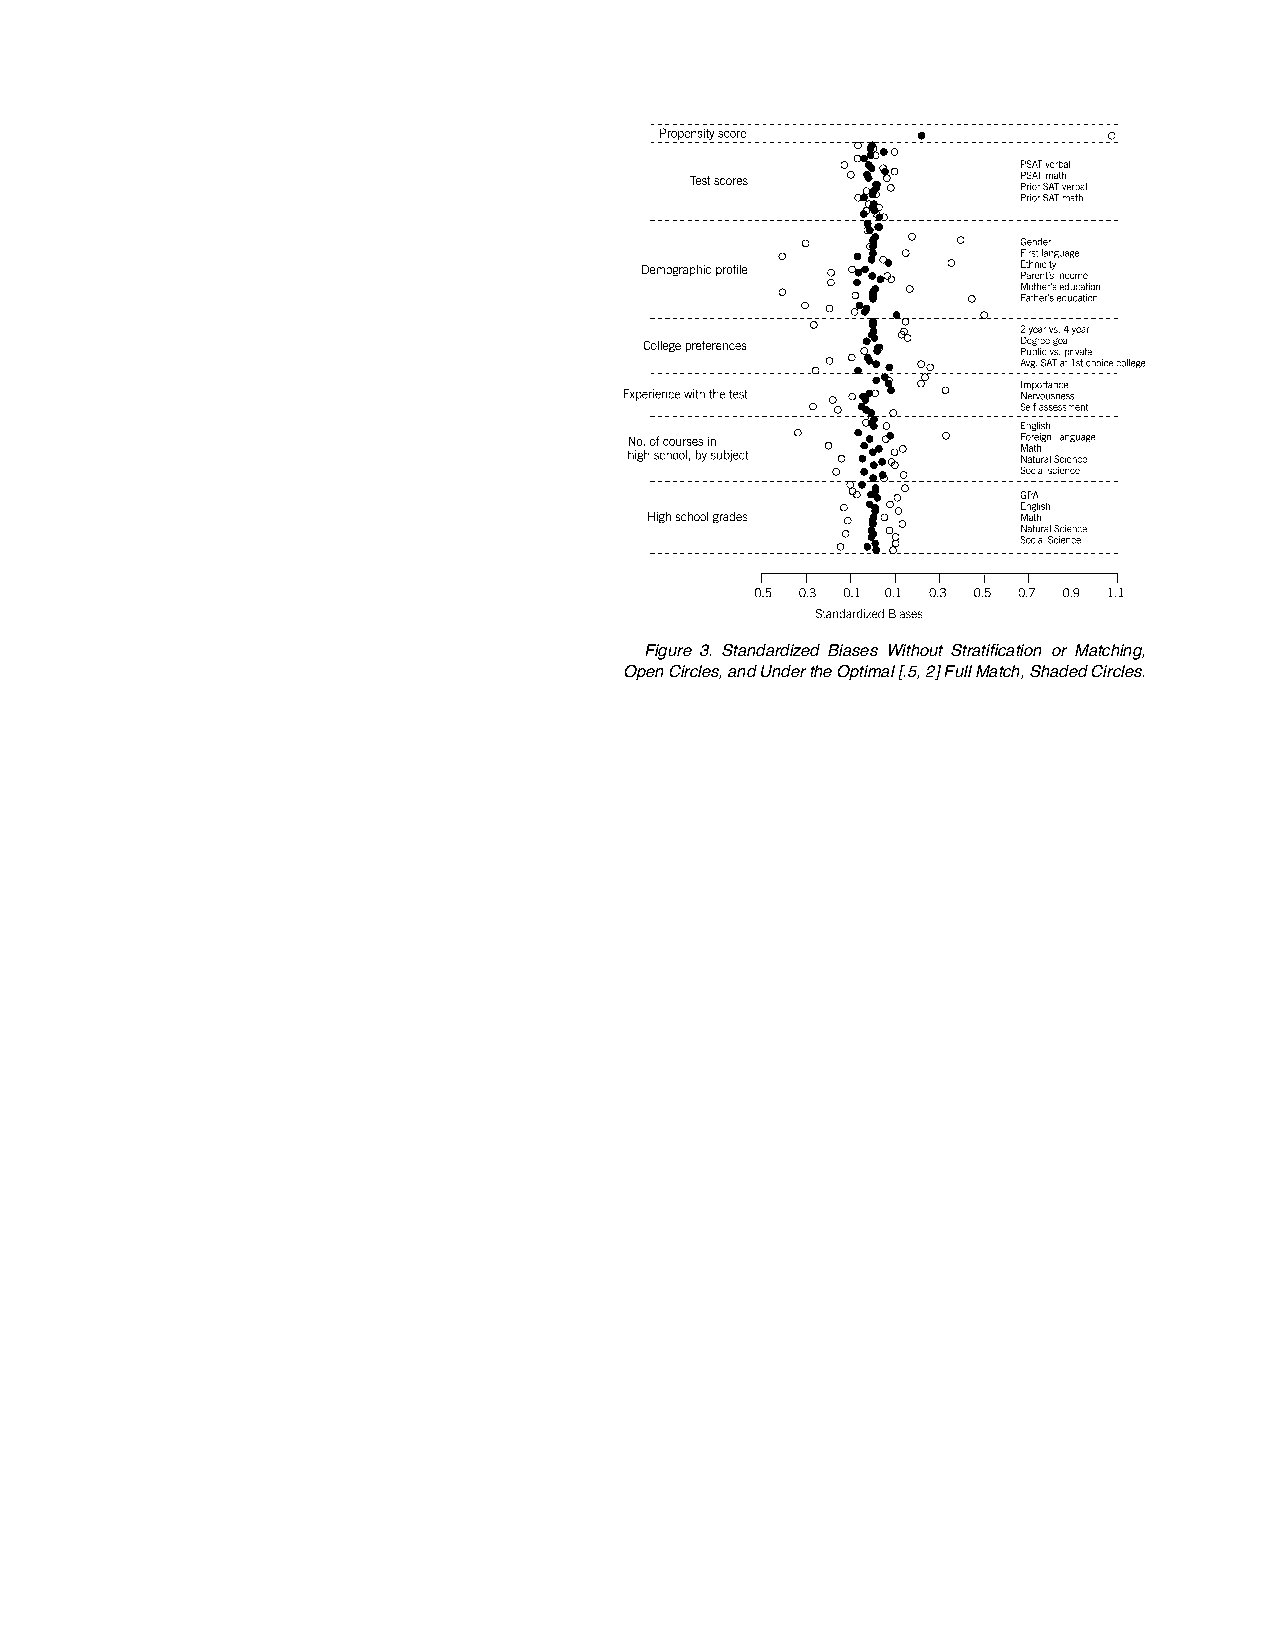
\includegraphics[width = .65 \linewidth]{images/hansen1.pdf}
%\end{figure}
%
%\end{frame}
%
%\begin{frame}{Balance Checks}
%
%\begin{figure}[ht] \centering
%    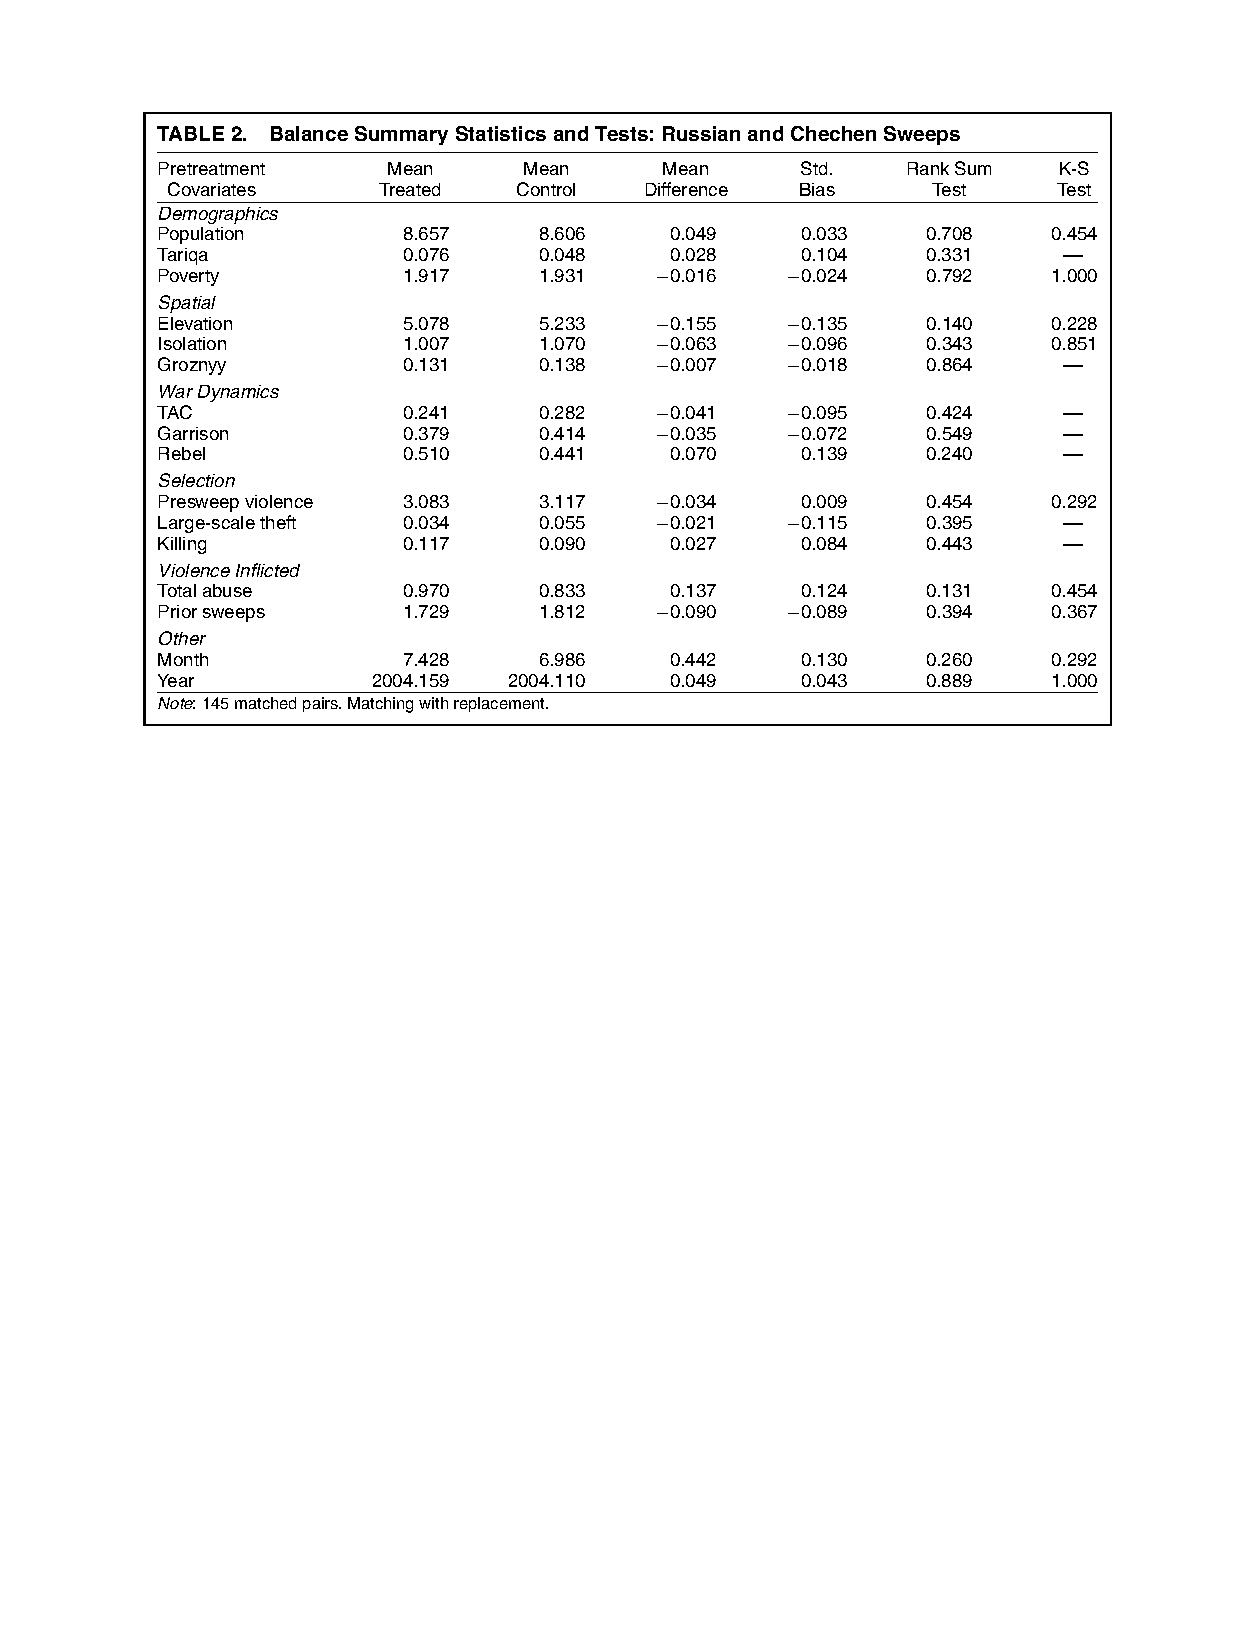
\includegraphics[width = .99 \linewidth]{images/lyall1.pdf}
%\end{figure}
%
%\end{frame}
%
%\begin{frame}{Variance of the Matching Estimator}
%
%\begin{itemize}
%\itemsep1pt\parskip0pt\parsep0pt
%\item
%  The sampling variance of the matching estimator (conditional on
%  covariates and treatment indicators) can be written as the following:
%  \[ \Var(\hat \tau_{ATT} | \mathbf{X}, \mathbf{D}) = \sum_{i=1}^{N} \lambda_i(\mathbf{X}, \mathbf{W}) \cdot \sigma^2_{D_i}(X_i)\]
%  where $\lambda_i(\mathbf{X}, \mathbf{W})$ is just a set of weights which
%  account for matching with replacement and multiple controls per
%  treatment unit. \pause
%\item
%  $\sigma^2_i$ is the unit level variance. Abadie and Imbens suggest
%  matching to estimate this quantity:
%
%  \begin{itemize}
%  \itemsep1pt\parskip0pt\parsep0pt
%  \item
%    Let $v(i)$ be the closest unit to $i$ with the same treatment
%    indicator ($D_{v(i)} = D_i$). The sample variance of the outcome
%    variable for these 2 units can be used to estimate
%    $\sigma^2_{D_i}(X_i)$:
%    \[ \hat \sigma^2_{D_i}(X_i) = (Y_i - Y_{v(i)})^2 / 2 \] 
%    \item Robust standard errors also available\pause
%  \end{itemize}
%\item
%  Do not use the bootstrap!
%\end{itemize}
%
%\end{frame}
%
%\begin{frame}[fragile]{Useful Matching Functions}
%
%The workhorse model is the \texttt{Match()} function in the
%\texttt{Matching} package:
%
%\small
%\begin{verbatim}
%Match(Y = NULL, Tr, X, Z = X, V = rep(1, length(Y)), 
%    estimand = "ATT", M = 1, BiasAdjust = FALSE, exact = NULL, 
%    caliper = NULL,  replace = TRUE, ties = TRUE, 
%    CommonSupport = FALSE, Weight = 1, Weight.matrix = NULL, 
%    weights = NULL, Var.calc = 0,  sample = FALSE, restrict = NULL, 
%    match.out = NULL, distance.tolerance = 1e-05, 
%    tolerance = sqrt(.Machine$double.eps), version = "standard") 
%\end{verbatim}
%
%Default distance metric (\texttt{Weight=1}) is normalized Euclidean distance
%
%\begin{itemize}
%\itemsep1pt\parskip0pt\parsep0pt
%\item
%  \texttt{MatchBalance(formu)} for balance checking
%\item
%  \texttt{GenMatch()} for genetic matching
%\end{itemize}
%
%\end{frame}
%
%\subsection{Propensity Scores}\label{propensity-scores}
%
%%\begin{frame}{Review: Law of Iterated Expectations}
%%
%%\begin{definition}
%%A very important property of conditional expectations is:
%%$$
%%\E[Y]=\E[\E[Y|X]]
%%$$
%%since $\E[Y|X]$ is a function of $X$, the outer expectation
%%is taken with respect to the distribution of $X$.
%%\end{definition}
%%
%%Example: \pause 
%%
%%Imagine $Y$=Support and $X$=gender $(1,0)$. Then, the law of iterated
%%expectations tells us: \[
%%\E[Y]=\pause \E[Y|X=1]\cdot \Pr(X=1) + \E[Y|X=0]\cdot \Pr(X=0).
%%\] This means: \medskip
%%\small
%%
%%\begin{tabular}{lcll}
%%Average Support &=& Average Support for men&$\times$ Proportion of men\\
%%               &+& Average Support for women&$\times$ Proportion of women.
%%\end{tabular}
%%
%%\end{frame}
%
%\begin{frame}{Identification with Propensity Scores}
%
%\begin{definition}
%Propensity score is defined as the selection probability conditional on the confounding variables:
%$\pi(X)=\Pr(D=1|X)$
%\end{definition}
%
%\begin{iass}
%\begin{enumerate}
%\item $(Y_1,Y_0) \indep D |X$ (selection on observables)
%\item $0<\Pr(D=1|X)<1$ with probability one (common support)
%\end{enumerate}
%\end{iass}
%
%\begin{ires}
%Under selection on observables we have $(Y_1,Y_0) \indep D| \pi(X)$, ie. conditioning
%on the propensity score is enough to have independence between the treatment indicator and potential outcomes. Implies substantial dimension reduction.
%\end{ires}
%
%\end{frame}
%
%\begin{frame}{Identification with Propensity Scores}
%
%\begin{Proof}
%\small
%Show that $\Pr(D = 1|Y_0, Y_1, \pi(X)) = \Pr(D = 1|\pi(X)) = \pi(X)$, implying
%independence of $(Y_0,Y_1)$ and $D$ conditional on $\pi(X)$.
%\begin{eqnarray*}
%\Pr(D=1|Y_1,Y_0,\pi(X))&=&\E[D|Y_1,Y_0,\pi(X)]\\ \pause
%&=&\E\left[\E[D|Y_1,Y_0,X]|Y_1,Y_0,\pi(X)\right] \mbox{ (LIE) }\\ \pause
%&=&\E\left[\E[D|X]|Y_1,Y_0,\pi(X)\right] \mbox{ (SOO) } \\\pause
%&=&\E\left[\pi(X)|Y_1,Y_0,\pi(X)\right] \\ \pause
%&=&\pi(X)
%\end{eqnarray*}
%Using a similar argument
%\begin{eqnarray*}
%\Pr(D=1|\pi(X))&=&\E[D|\pi(X)]=\E[\E[D|X]|\pi(x)]\\ \pause
%&=&\E[\pi(X)|\pi(X)]=\pi(X)
%\end{eqnarray*}
%therefore $\Pr(D=1|Y_1,Y_0,\pi(X))=\Pr(D=1|\pi(X))$
%\end{Proof}
%
%\end{frame}
%
%\begin{frame}{Matching on the Propensity Score}
%
%\begin{corollary} If $(Y_1,Y_0) \indep D|X$, then
%\begin{eqnarray*}
%\E[Y|D=1,\pi(X)=\bar{\pi}]-\E[Y|D=0,\pi(X)=\bar{\pi}]&=&\\
%\E[Y_1-Y_0|\pi(X)=\bar{\pi}]
%\end{eqnarray*}
%\end{corollary}
%
%Suggests a two step procedure to estimate causal effects under selection
%on observables:
%
%\begin{enumerate}
%\def\labelenumi{\arabic{enumi}.}
%\itemsep1pt\parskip0pt\parsep0pt
%\item
%  Estimate the propensity score $\pi(X)=P(D=1|X)$ (eg. using
%  logit/probit regression, machine learning methods, etc) \pause
%\item
%  Match or subclassify on propensity score.
%\end{enumerate}
%
%\end{frame}
%
%\begin{frame}{Estimating the Propensity Score}
%
%\begin{itemize}
%\itemsep1pt\parskip0pt\parsep0pt
%\item
%  Given selection on observables we have $(Y_1,Y_0) \indep D|\pi(X)$
%  which implies the balancing property of the propensity score: \[
%    \Pr(X|D=1,\pi(X))=\Pr(X|D=0,\pi(X))
%    \] \pause
%\item
%  We can use this to check if our estimated propensity score actually
%  produces balance:
%  $P(X|D=1,\widehat{\pi}(X))=P(X|D=0,\widehat{\pi}(X))$ \pause
%\item
%  To properly model the assignment mechanism, we need to include
%  important confounders correlated with treatment and outcome
%\item
%  Need to find the correct functional form, miss-specified propensity
%  scores can lead to bias. Any methods can be used (probit, logit, etc.)
%\item
%  Estimate $\mapsto$ Check Balance $\mapsto$ Re-estimate $\mapsto$ Check
%  Balance
%\end{itemize}
%
%\end{frame}
%
%\begin{frame}[fragile]{Example: Blattman (2010)}
%
%\footnotesize
%
%%\begin{Shaded}
%%\begin{Highlighting}[]
%%\NormalTok{pscore.fmla <-}\StringTok{ }\KeywordTok{as.formula}\NormalTok{(}\KeywordTok{paste}\NormalTok{(}\StringTok{"abd~"}\NormalTok{,}\KeywordTok{paste}\NormalTok{(}\KeywordTok{names}\NormalTok{(covar),}\DataTypeTok{collapse=}\StringTok{"+"}\NormalTok{)))}
%%\NormalTok{abd <-}\StringTok{ }\NormalTok{data$abd}
%%\NormalTok{pscore_model <-}\StringTok{ }\KeywordTok{glm}\NormalTok{(pscore.fmla, }\DataTypeTok{data =} \NormalTok{data, }
%%  \DataTypeTok{family =} \KeywordTok{binomial}\NormalTok{(}\DataTypeTok{link =} \NormalTok{logit))}
%%\NormalTok{pscore <-}\StringTok{ }\KeywordTok{predict}\NormalTok{(pscore_model, }\DataTypeTok{type =} \StringTok{"response"}\NormalTok{)}
%%\end{Highlighting}
%%\end{Shaded}
%
%\centering
%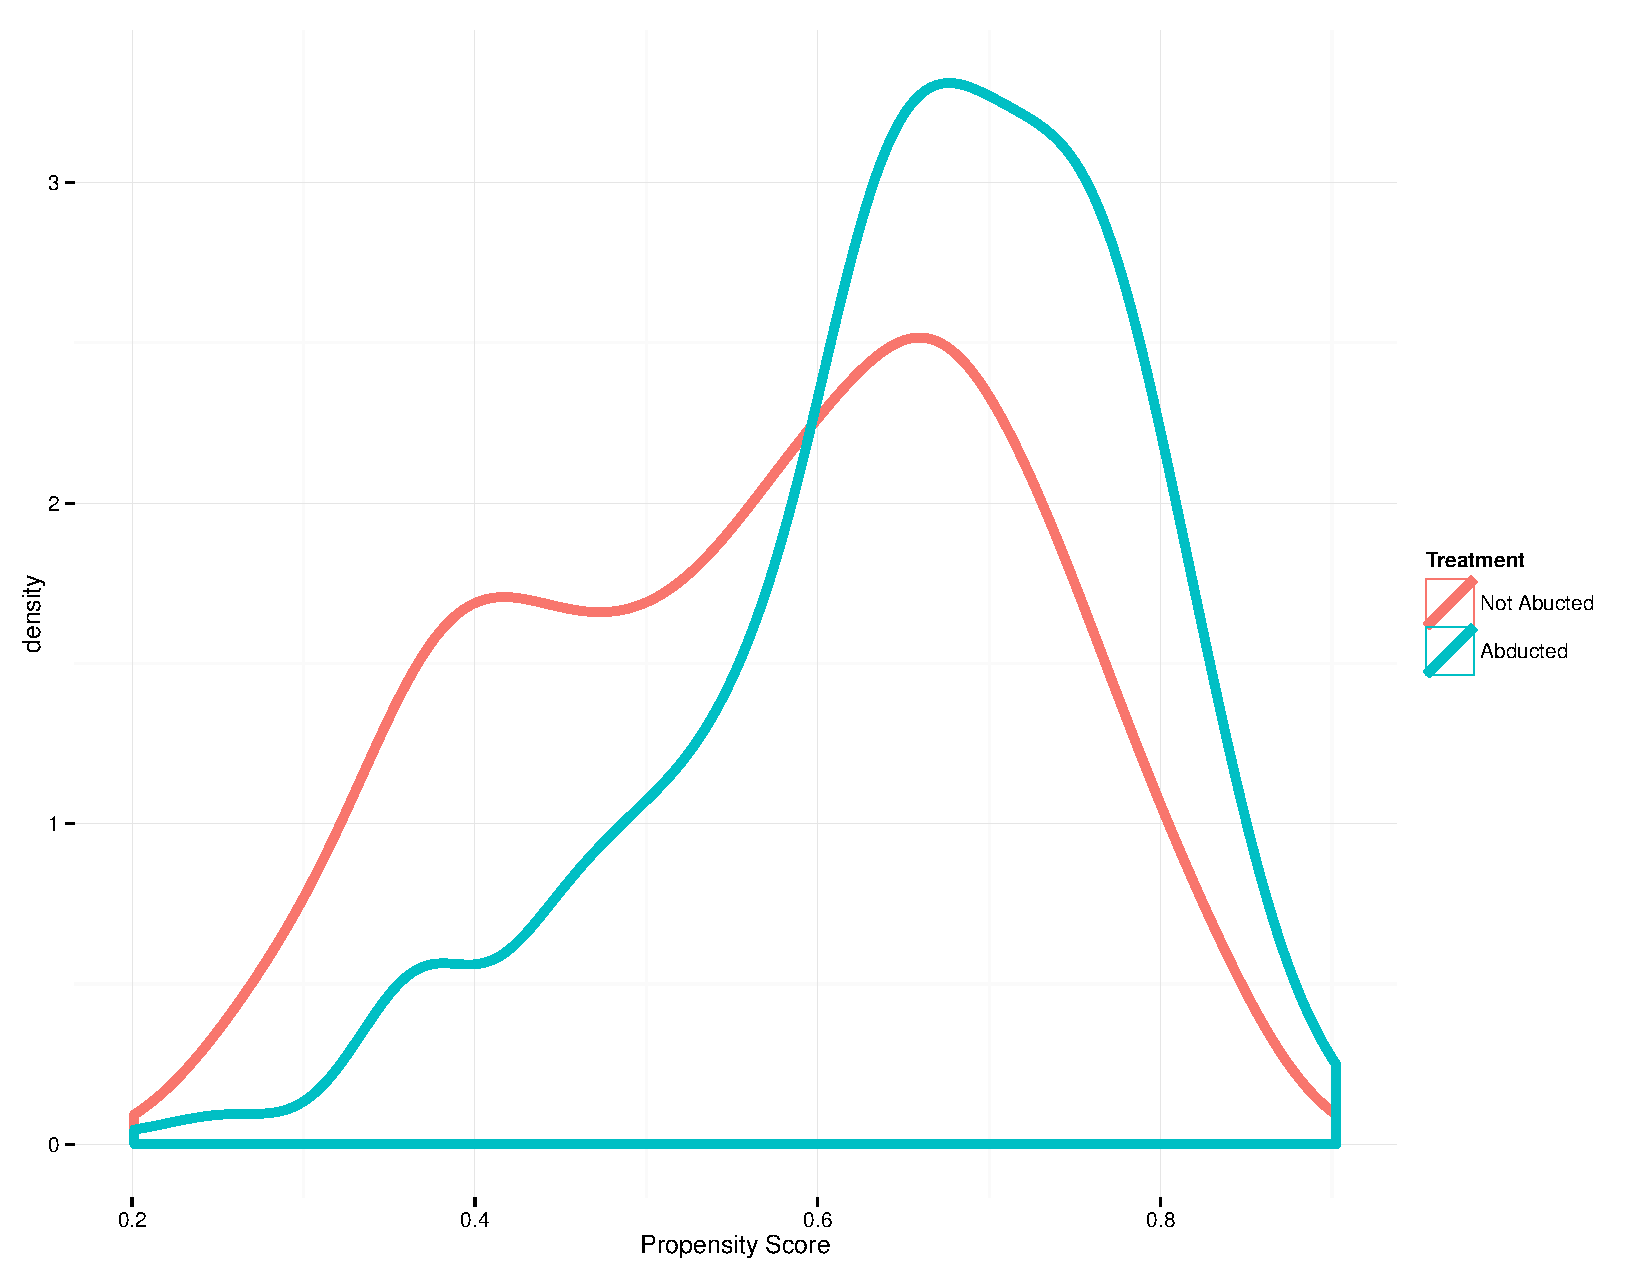
\includegraphics[height = 2.4in]{images/blattman_pscore.pdf}
%\end{frame}
%
%\begin{frame}[fragile]{Blattman (2010): Match on the Propensity Score}
%
%\footnotesize
%
%%\begin{Shaded}
%%\begin{Highlighting}[]
%%\NormalTok{match.pscore <-}\StringTok{ }\KeywordTok{Match}\NormalTok{(}\DataTypeTok{Tr=}\NormalTok{abd, }\DataTypeTok{X=}\NormalTok{pscore, }\DataTypeTok{M=}\DecValTok{1}\NormalTok{, }\DataTypeTok{estimand=}\StringTok{"ATT"}\NormalTok{)}
%%\end{Highlighting}
%%\end{Shaded}
%%
%\centering
%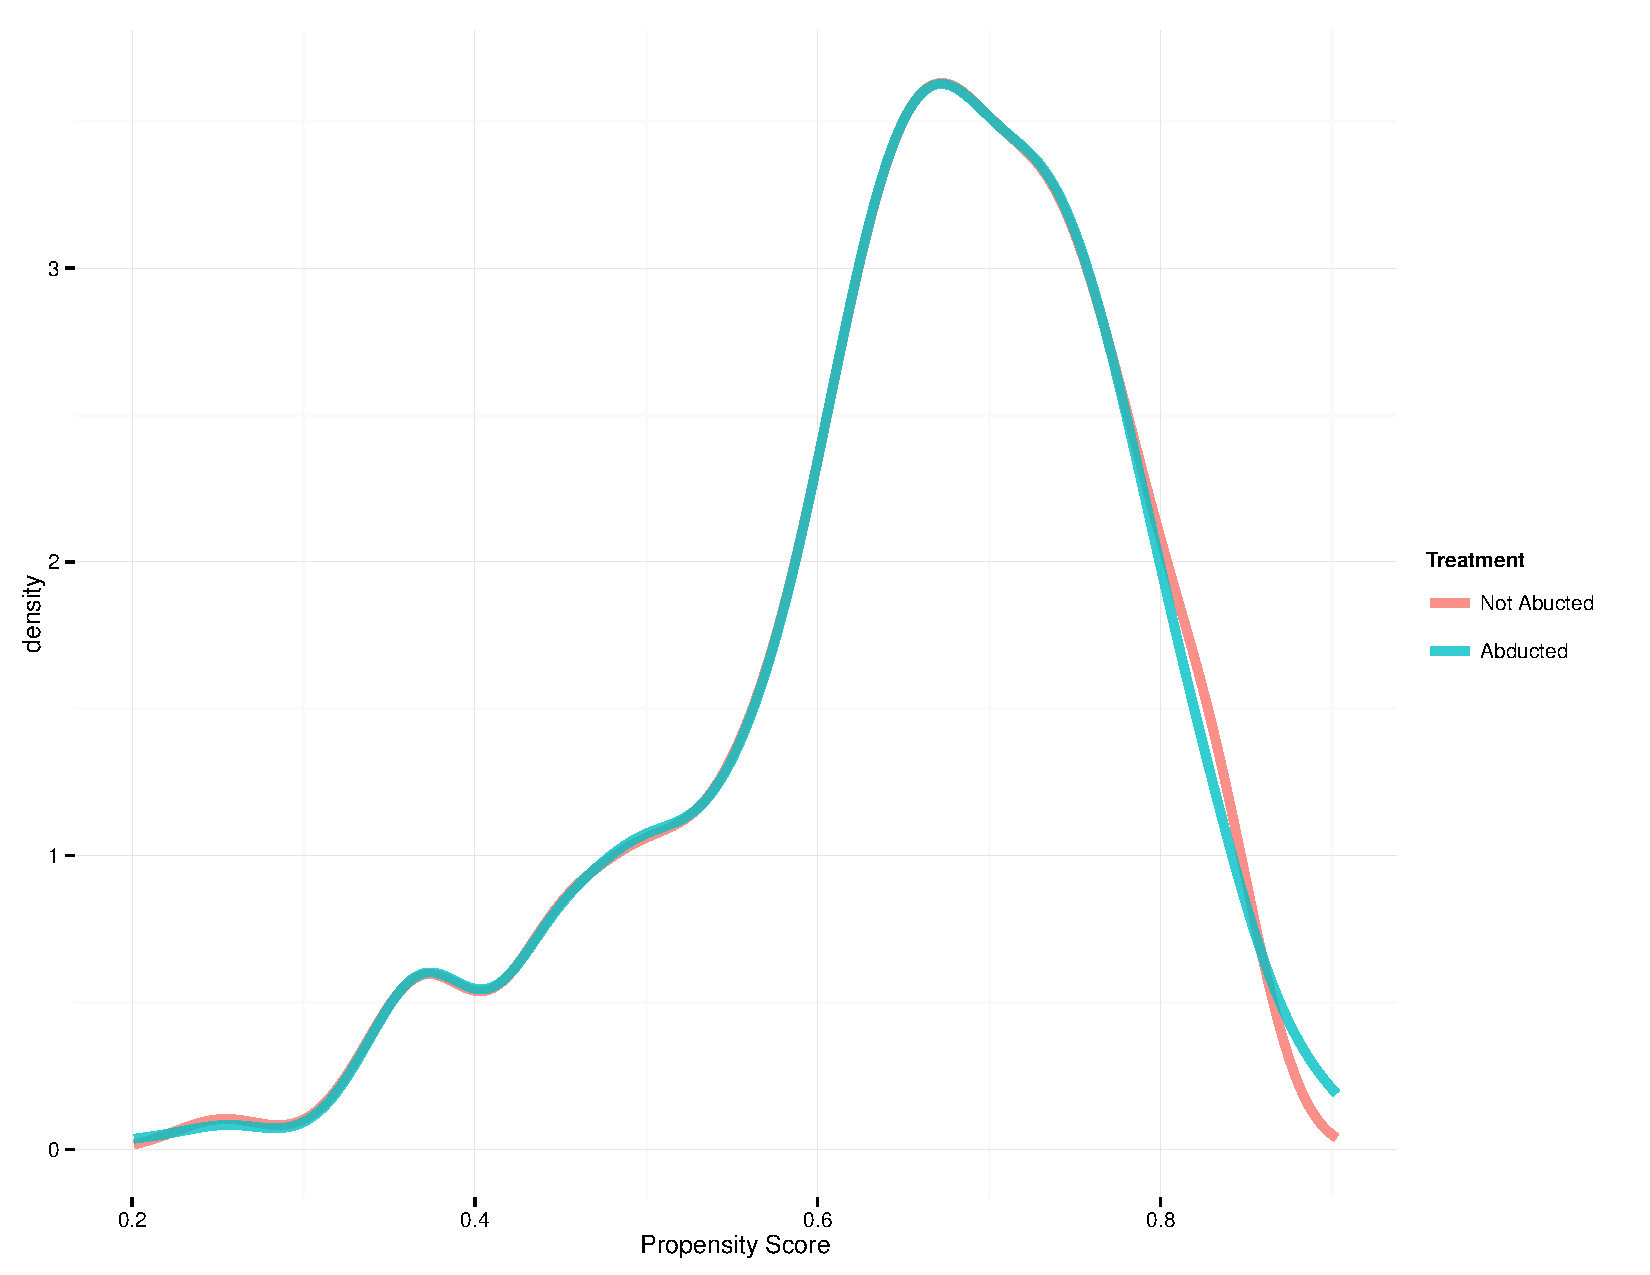
\includegraphics[height = 3in]{images/blattman_pscore_matching.pdf}
%
%\end{frame}
%
%%\begin{frame}[fragile]{Blattman (2010): Check Balance}
%%
%%\footnotesize
%%
%%\begin{Shaded}
%%\begin{Highlighting}[]
%%\NormalTok{match.pscore <-}
%%\NormalTok{+}\StringTok{ }\KeywordTok{MatchBalance}\NormalTok{(abd ~}\StringTok{ }\NormalTok{age, }\DataTypeTok{data=}\NormalTok{data, }\DataTypeTok{match.out =} \NormalTok{match.pscore)}
%%
%%\NormalTok{**}\ErrorTok{***}\StringTok{ }\NormalTok{(V1) age **}\ErrorTok{***}
%%\StringTok{                       }\NormalTok{Before Matching     After Matching}
%%\NormalTok{mean treatment........     }\FloatTok{21.366}          \FloatTok{21.366} 
%%\NormalTok{mean control..........     }\FloatTok{20.151}          \FloatTok{20.515} 
%%\NormalTok{std mean diff.........     }\FloatTok{24.242}          \FloatTok{16.976} 
%%
%%\NormalTok{var }\KeywordTok{ratio} \NormalTok{(Tr/Co).....     }\FloatTok{1.0428}         \FloatTok{0.98412} 
%%\NormalTok{T-test p-value........  }\FloatTok{0.0012663}       \FloatTok{0.0034409} 
%%\NormalTok{KS Bootstrap p-value..      }\FloatTok{0.016}           \FloatTok{0.034} 
%%\NormalTok{KS Naive p-value......   }\FloatTok{0.024912}        \FloatTok{0.070191} 
%%\NormalTok{KS Statistic..........    }\FloatTok{0.11227}        \FloatTok{0.077899} 
%%\end{Highlighting}
%%\end{Shaded}
%%
%%\end{frame}
%
%%\begin{frame}[fragile]{Blattman (2010): Mahalanobis Distance Matchng}
%%\footnotesize
%%
%%\begin{Shaded}
%%\begin{Highlighting}[]
%%\NormalTok{match.mah <-}\StringTok{ }\KeywordTok{Match}\NormalTok{(}\DataTypeTok{Tr=}\NormalTok{abd, }\DataTypeTok{X=}\NormalTok{covar, }\DataTypeTok{M=}\DecValTok{1}\NormalTok{, }\DataTypeTok{estimand=}\StringTok{"ATT"}\NormalTok{, }\DataTypeTok{Weight =} \DecValTok{3}\NormalTok{)}
%%\KeywordTok{MatchBalance}\NormalTok{(abd ~}\StringTok{ }\NormalTok{age, }\DataTypeTok{data=}\NormalTok{data, }\DataTypeTok{match.out =} \NormalTok{match.mah)}
%%
%%\NormalTok{**}\ErrorTok{***}\StringTok{ }\NormalTok{(V1) age **}\ErrorTok{***}
%%\StringTok{                       }\NormalTok{Before Matching     After Matching}
%%\NormalTok{mean treatment........     }\FloatTok{21.366}          \FloatTok{21.366} 
%%\NormalTok{mean control..........     }\FloatTok{20.151}          \FloatTok{21.154} 
%%\NormalTok{std mean diff.........     }\FloatTok{24.242}          \FloatTok{4.2314} 
%%
%%\NormalTok{var }\KeywordTok{ratio} \NormalTok{(Tr/Co).....     }\FloatTok{1.0428}          \FloatTok{1.0336} 
%%\NormalTok{T-test p-value........  }\FloatTok{0.0012663}      \FloatTok{3.0386e-05} 
%%\NormalTok{KS Bootstrap p-value..      }\FloatTok{0.008}           \FloatTok{0.798} 
%%\NormalTok{KS Naive p-value......   }\FloatTok{0.024912}         \FloatTok{0.94687} 
%%\NormalTok{KS Statistic..........    }\FloatTok{0.11227}        \FloatTok{0.034261} 
%%\end{Highlighting}
%%\end{Shaded}
%%\end{frame}
%
%%\begin{frame}[fragile]{Blattman (2010): Genetic Matching}
%%
%%\footnotesize
%%
%%\begin{Shaded}
%%\begin{Highlighting}[]
%%\NormalTok{genout <-}\StringTok{ }\KeywordTok{GenMatch}\NormalTok{(}\DataTypeTok{Tr=}\NormalTok{abd,}\DataTypeTok{X=}\NormalTok{covar,}\DataTypeTok{BalanceMatrix=}\NormalTok{covar,}\DataTypeTok{estimand=}\StringTok{"ATT"}\NormalTok{,}
%%                  \DataTypeTok{pop.size=}\DecValTok{1000}\NormalTok{)}
%%\NormalTok{match.gen <-}\StringTok{ }\KeywordTok{Match}\NormalTok{(}\DataTypeTok{Tr=}\NormalTok{abd, }\DataTypeTok{X=}\NormalTok{covar,}\DataTypeTok{M=}\DecValTok{1}\NormalTok{,}\DataTypeTok{estimand=}\StringTok{"ATT"}\NormalTok{,}\DataTypeTok{Weight.matrix=}\NormalTok{genout)}
%%\NormalTok{gen.bal <-}\StringTok{ }\KeywordTok{MatchBalance}\NormalTok{(abd~age,}\DataTypeTok{match.out=}\NormalTok{match.gen,}\DataTypeTok{data=}\NormalTok{covar)}
%%
%%\NormalTok{**}\ErrorTok{***}\StringTok{ }\NormalTok{(V1) age **}\ErrorTok{***}
%%\StringTok{                       }\NormalTok{Before Matching     After Matching}
%%\NormalTok{mean treatment........     }\FloatTok{21.366}          \FloatTok{21.366} 
%%\NormalTok{mean control..........     }\FloatTok{20.151}          \FloatTok{21.225} 
%%\NormalTok{std mean diff.........     }\FloatTok{24.242}          \FloatTok{2.8065} 
%%
%%\NormalTok{var }\KeywordTok{ratio} \NormalTok{(Tr/Co).....     }\FloatTok{1.0428}          \FloatTok{1.1337} 
%%\NormalTok{T-test p-value........  }\FloatTok{0.0012663}         \FloatTok{0.21628} 
%%\NormalTok{KS Bootstrap p-value..      }\FloatTok{0.008}           \FloatTok{0.454} 
%%\NormalTok{KS Naive p-value......   }\FloatTok{0.024912}         \FloatTok{0.68567} 
%%\NormalTok{KS Statistic..........    }\FloatTok{0.11227}        \FloatTok{0.046512} 
%%\end{Highlighting}
%%\end{Shaded}
%%
%%\end{frame}
%
%\begin{frame}{Weighting on the Propensity Score}
%
%\small
%Provided that the relevant moments exists, if $Y_1,Y_0\indep D |X$, then
%
%\begin{eqnarray*}
%\tau_{ATE}&=&\E[Y_1-Y_0]=\E\left[
%Y\cdot \frac{D-\pi(X)}{\pi(X)\cdot (1-\pi(X))}
%\right]\\
%\tau_{ATT}&=&\E[Y_1-Y_0|D=1]=\frac{1}{P(D=1)}\cdot \E\left[
%Y\cdot \frac{D-\pi(X)}{1-\pi(X)}
%\right]
%\end{eqnarray*}
%
%\begin{Proof}
%\scriptsize Consider
%\begin{eqnarray*}
%&&\E\left[\left.
%Y \frac{D-\pi(X)}{\pi(X) (1-\pi(X))}\right| X \right]\\
%&=& \E\left[\left.\frac{Y}{\pi(X)} \right|X, D=1 \right] \pi(X) + \E\left[\left.\frac{-Y}{1-\pi(X)}\right|X, D=0\right] (1-\pi(X))\\
%&=& \E[Y|X, D=1] - \E[Y|X, D=0]
%\end{eqnarray*}
%And the results of the proposition follow from integration over $\Pr(X)$ and $\Pr(X|D=1)$.
%\end{Proof}
%
%\end{frame}
%
%\begin{frame}{Weighting on the Propensity Score}
%
%\small
%
%\begin{eqnarray*}
%\tau_{ATE}&=&\E[Y_1-Y_0]=\E\left[
%Y\cdot \frac{D-\pi(X)}{\pi(X)\cdot (1-\pi(X))}
%\right]\\
%\tau_{ATT}&=&\E[Y_1-Y_0|D=1]=\frac{1}{\Pr(D=1)}\cdot \E\left[
%Y\cdot \frac{D-\pi(X)}{1-\pi(X)}
%\right]
%\end{eqnarray*}
%
%How do we estimate this? \pause Analogy principle suggest a two step
%procedure:
%
%\begin{enumerate}
%\def\labelenumi{\arabic{enumi}.}
%\itemsep1pt\parskip0pt\parsep0pt
%\item
%  Estimate the propensity score ($\widehat{\pi}(X)$)
%\item
%  Use sample averages and the estimated propensity score to produce
%  analog estimators of $\tau_{ATE}$ and $\tau_{ATT}$:
%
%  \begin{eqnarray*}
%  \widehat{\tau}_{ATE}&=&\frac{1}{N} \sum_{i=1}^N
%  Y_i\cdot \frac{D_i-\widehat{\pi}(X_i)}{\widehat{\pi}(X_i)\cdot
%  (1-\widehat{\pi}(X_i))},\\
%  \widehat{\tau}_{ATT}&=&\frac{1}{N} \sum_{i=1}^N
%  Y_i\cdot \frac{D_i-\widehat{\pi}(X_i)}{1-\widehat{\pi}(X)}
%  \end{eqnarray*}
%\end{enumerate}
%
%\end{frame}


\end{document}